\documentclass[12pt,a4paper]{amsart}
\usepackage[utf8]{inputenc}
\usepackage[T1]{fontenc}
\usepackage{amsmath,amssymb,amsthm}
\usepackage{booktabs}
\usepackage{graphicx}
\usepackage{enumitem}
\usepackage[margin=1in]{geometry}
\usepackage{xcolor}
\usepackage{float}
\usepackage{tikz}
\usetikzlibrary{arrows.meta,positioning,calc}
\usepackage{hyperref}
\hypersetup{colorlinks=true,linkcolor=blue!60!black,citecolor=blue!60!black,urlcolor=blue!60!black,
  pdftitle={Prime polynomials in Legendre intervals over F(2k)[t], IV: point counts on hexad modular curves, Brown invariants of Witt sheaves, and the constant X},
  pdfauthor={Ruqing Chen}}

\newtheorem{theorem}{Theorem}[section]
\newtheorem{proposition}[theorem]{Proposition}
\newtheorem{lemma}[theorem]{Lemma}
\newtheorem{corollary}[theorem]{Corollary}
\newtheorem{conjecture}[theorem]{Conjecture}
\newtheorem{target}[theorem]{Target Theorem}
\theoremstyle{definition}
\newtheorem{definition}[theorem]{Definition}
\newtheorem{remark}[theorem]{Remark}
\newtheorem{example}[theorem]{Example}
\newtheorem{question}[theorem]{Question}

\newcommand{\F}{\mathbb{F}}
\newcommand{\Z}{\mathbb{Z}}
\newcommand{\Q}{\mathbb{Q}}
\newcommand{\C}{\mathbb{C}}
\newcommand{\G}{\mathcal{G}}
\newcommand{\Tr}{\operatorname{Tr}}
\newcommand{\Var}{\operatorname{Var}}
\newcommand{\Sp}{\operatorname{Sp}}
\newcommand{\GL}{\operatorname{GL}}
\newcommand{\Br}{\operatorname{Br}}
\newcommand{\Arf}{\operatorname{Arf}}
\newcommand{\sgn}{\operatorname{sgn}}
\newcommand{\eps}{\varepsilon}
\newcommand{\Kk}{\mathcal{K}}
\newcommand{\qq}{\mathfrak{q}}
\newcommand{\Spp}{S''}
\newcommand{\Tw}{\mathsf{T}}
\newcommand{\todo}[1]{\textcolor{red!70!black}{[#1]}}
\emergencystretch=2em
\allowdisplaybreaks
\raggedbottom

\title[Legendre intervals in even characteristic, IV]{Prime polynomials in Legendre intervals over \texorpdfstring{$\F_{2^k}[t]$}{F(2k)[t]}, IV:\texorpdfstring{\\}{ }point counts on hexad modular curves, Brown invariants of Witt sheaves, and the constant \texorpdfstring{$X$}{X}}

\author{Ruqing Chen}
\address{GUT Geoservice Inc., Montreal, Canada}
\email{ruqing@hotmail.com}
\thanks{DOI 10.5281/zenodo.23299284. Part~I: DOI 10.5281/zenodo.23225896; Part~II: DOI 10.5281/zenodo.23252762; Part~III: DOI 10.5281/zenodo.23290724. Code and data for this paper: \url{https://github.com/Ruqing1963/legendre-intervals-part4}.}
\date{\today}

\begin{document}

\begin{abstract}
Let $q=2^k$ with $k$ odd. Part~III reduced the closed form $X=q^6+q^5$ of the second constant of the degree-$6$ Legendre variance to two statements about the sextic family $B_\lambda=\lambda_5^2u^6+\lambda_3^2u^2+\lambda_5u+1$ whose roots form the hexad of $\ker L'_\lambda$: the polynomial frequencies of its eleven factorisation types over $\F_q$, and the signs of the Gauss sums $s_4$, $s_6$ of explicit $\Z/4$-valued quadratic forms on $\F_{q^4}$, $\F_{q^6}$. This paper proves three structural theorems about these Gauss sums and uses them to settle the signs in the two classes of order~$4$. The \emph{hexad formula} expresses $s_{2m}$, a sum over $\F_{q^{2m}}$, as $q^m$ times a signed sum of at most sixteen fourth roots of unity indexed by the $\F_{q^m}$-rational points of the coset $T_\lambda'^{-1}(1)$ (the six roots and the ten synthematic totals), with sign $+$ at roots and $-$ at totals. The \emph{trace parity theorem} determines the absolute trace of every such point: $\Tr_{q^m/2}(w)\equiv mk+\dim(\Kk_\lambda\cap\F_{q^m})\pmod2$; for $m=1$ it says that a rational root of $B_\lambda$ has trace $0$ or $1$ according to the Frobenius class. Together with an elementary count on the sixteen-point configuration of roots and totals they determine the signs in nine of the eleven classes: $s_4=+4q^2$ throughout the classes $1^6$, $2^3$; $s_4=\pm4q^2$ on complementary half-spaces of $\lambda_1$ in the classes $2\,1^4$, $2^21^2$; $s_4\in\{0,+4q^2\}$, respectively $\{0,-4q^2\}$, nonzero exactly on an explicit affine hyperplane, in the classes $4\,1^2$, $4\,2$, hence $W'=+2q^7$ and $-2q^7$ as conjectured since Part~II; and $\Spp=+4q^6$ throughout the classes $3\,1^3$ and $3^2$. The class $6$ is settled under a single Witt identity verified for $q\le32$, and only the class $3\,2\,1$ remains open. The hyperplane parameter $\kappa_0$ of the order-$4$ classes is given in closed form in the ground-field data of the quartic cofactor; contrary to what the data at $q=8$ suggested, it is not constant on the class. For the factorisation counts, every moment $\sum_\lambda N_m(B_\lambda)$ is expressed through Gauss sums of Gold-type forms on the trace-zero hyperplane of $\F_{q^m}$; the identity is proved for all $m$, the third moment $2q^2-3q-1$ is verified for $q\le128$, and an explicit nonsingular $11\times11$ system of pure and mixed moments whose unique solution is the conjectured table of class counts is written down.
\end{abstract}

\maketitle
\tableofcontents

\section{Introduction and main results}\label{sec:intro}

\subsection{Where Part III left the problem}
Parts I--III \cite{Chen,ChenII,ChenIII} study the variance of the prime-power count $\Psi$ over Legendre intervals $\{f^2+s:\deg s\le d\}$ in $\F_q[t]$, $q=2^k$, the function-field analogue of the problem of Keating and Rudnick \cite{KeatingRudnick} in the even-characteristic regime where the Weil-II/equidistribution route of Katz \cite{KatzKR,KatzEKR} must be replaced by exact evaluations. At $d=6$ the variance is an explicit function of three constants $A_6$, $X$, $Y$ (Part~II); $A_6=q^9+(q-1)q^5$ is proved for odd $k$, $Y=q^3m_k$ has no elementary closed form, and
\begin{equation}\label{eq:X}
X=q^{-3}\sum_{\lambda_3,\lambda_5\in\F_q}W'(\lambda_3,\lambda_5),\qquad W'(\lambda_3,\lambda_5)=\sum_{\lambda_1\in\F_q}\Spp(\lambda_1,\lambda_3,\lambda_5),
\end{equation}
where $\Spp(\lambda)=\sum_{x\in\F_{q^{12}}}i^{\qq_\lambda(x)}$ is the Gauss sum of the $\Z/4$-valued quadratic form
\[
\qq_\lambda(x)=\Tw_{12k}(x)+2\Tr_{q^{12}/2}(\lambda_5x^5+\lambda_3x^3+\lambda_1x),\qquad \Tw_n(x)=\Tr_{W_2(\F_{2^n})/\Z/4}[x],
\]
$[x]$ the Teichm\"uller representative in the Witt vectors of length two (the trace of Frobenius on a rank-four Witt--Artin--Schreier sheaf in the sense of Brylinski \cite{Brylinski} and Katz \cite{KatzKR}; the quadratic forms with values in $\Z/4$ and their Gauss sums are those of Brown \cite{Brown}). Part~III proved that for $\lambda_5\ne0$ the radical $\Kk_\lambda$ of $\qq_\lambda$ is governed by the hexad $\{r_1,\dots,r_6\}$ of roots of
\[
B_\lambda(u)=\lambda_5^2u^6+\lambda_3^2u^2+\lambda_5u+1,\qquad \Kk_\lambda=\ker T'_\lambda=\{0\}\cup\{r_i+r_j\},\qquad T'_\lambda(r_i)=1,
\]
where $T'_\lambda(x)=\lambda_5x^4+\lambda_3x^2+x+(\lambda_3x)^{1/2}+(\lambda_5x)^{1/4}$ is the polar operator of $\qq_\lambda$, i.e.
\begin{equation}\label{eq:polar}
\qq^{(m)}_\lambda(x+y)=\qq^{(m)}_\lambda(x)+\qq^{(m)}_\lambda(y)+2\Tr_{q^m/2}\bigl(y\,T'_\lambda(x)\bigr)\qquad(x,y\in\F_{q^m}),
\end{equation}
for the forms $\qq^{(m)}_\lambda(x)=\Tw_{mk}(x)+2\Tr_{q^m/2}(\lambda_5x^5+\lambda_3x^3+\lambda_1x)$ on $\F_{q^m}$ with Gauss sums $s_m(\lambda)=\sum_{x\in\F_{q^m}}i^{\qq^{(m)}_\lambda(x)}$. The Frobenius $\sigma$ acts on $\Kk_\lambda$ through $S_6\cong\Sp_4(\F_2)$ \cite{Atlas} as the permutation $\pi_\lambda$ of the roots, the coset $T_\lambda'^{-1}(1)=r_1+\Kk_\lambda$ consists of the six roots and the ten \emph{synthematic totals} $r_i+r_j+r_l$ ($\{i,j\},\{l,\cdot\}$ running over the three duads of a syntheme), and $W'$ is determined by the class of $\pi_\lambda$ together with the signs of certain small-field Gauss sums. Precisely (Part~III, Theorems~6.9, 6.12, 6.14 and Corollary~1.5), with $N_0$ the order of $\pi_\lambda$:
\begin{itemize}[leftmargin=2em]
\item class $5\,1$: $W'=-q^7$ (proved);
\item $N_0\mid4$ (classes $1^6$, $2\,1^4$, $2^21^2$, $2^3$, $4\,1^2$, $4\,2$): $\Spp(\lambda)=q^4s_4(\lambda)$ with $s_4(\lambda)\in\{0,\pm4q^2\}$ (proved); for $N_0=4$ the set $\{\lambda_1:s_4\ne0\}$ is empty or the affine hyperplane $\Tr_{q/2}(\lambda_1\tau_0)=\kappa_0$, $\tau_0=r_5+r_6$ (proved); the \emph{signs} were conjectural;
\item $N_0\in\{3,6\}$ (classes $3\,1^3$, $3^2$, $3\,2\,1$, $6$): $\Spp(\lambda)=\pm4q^6$ for all $\lambda_1$ (proved); the sign is $+$ when $s_3\ne0$ and $N_0=3$ (proved), and is otherwise conjectural.
\end{itemize}

\begin{target}[Part~III, Conjecture~5.3]\label{tgt:counts}
For odd $k$ the number of $(\lambda_3,\lambda_5)\in\F_q^\times\times\F_q^\times$ with $B_\lambda$ of class $C$ is the polynomial $n_C(q)$ of Part~III, Table~2:
\[
\begin{array}{llll}
1^6:\ \tfrac{(q-2)(q-8)}{720}, & 2\,1^4:\ \tfrac{(q-2)(q-8)}{48}, & 2^21^2:\ \tfrac{q(q-2)}{16}, & 2^3:\ \tfrac{(q-2)(q-8)}{48},\\[0.5ex]
3\,1^3:\ \tfrac{(q+1)(q-2)}{18}, & 3^2:\ \tfrac{(q+1)(q-2)}{18}, & 3\,2\,1:\ \tfrac{(q+1)(q-2)}{6}, & 4\,1^2:\ \tfrac{(q-2)(q-4)}{8},\\[0.5ex]
4\,2:\ \tfrac{q(q-2)}{8}, & 5\,1:\ \tfrac{q^2+1}{5}, & 6:\ \tfrac{(q+1)(q-2)}{6}, &
\end{array}
\]
and for $\lambda_3=0$ the classes $2^3$, $4\,1^2$, $6$ occur $(q-2)/6$, $(q-2)/2$, $(q+1)/3$ times (the latter is a theorem).
\emph{Status: verified for $q\le512$; the relations of Part~III, Corollary~5.1, and the moment identities of Section~\ref{sec:moments} are proved.}
\end{target}

\begin{target}[Part~III, Conjecture~6.17]\label{tgt:signs}
For odd $k$: $s_4(\lambda)=+4q^2$ for all $\lambda_1$ in the classes $1^6$, $2^3$; $s_4(\lambda)=\pm4q^2$ for $q/2$ values of $\lambda_1$ each in the classes $2\,1^4$, $2^21^2$; $s_4(\lambda)\in\{0,+4q^2\}$ in the class $4\,1^2$ and $\in\{0,-4q^2\}$ in the class $4\,2$, nonzero for $q/2$ values of $\lambda_1$; $\Spp(\lambda)=+4q^6$ for all $\lambda_1$ in the classes $3\,1^3$, $3^2$, $6$, and $=\pm4q^6$ in equal numbers in the class $3\,2\,1$.
\emph{Status: proved in this paper for the classes $1^6$, $2\,1^4$, $2^21^2$, $2^3$ (Theorem~\ref{thm:N0div2}), $4\,1^2$, $4\,2$ (Theorem~\ref{thm:order4}), $3\,1^3$, $3^2$ (Theorem~\ref{thm:N0div6}), and for the class $6$ under the hypothesis \textup{(H)} of \eqref{eq:H}, verified at $q=8,32$; the class $3\,2\,1$ remains verified only (all $\lambda$ at $q=8$, and through $W'$ for $q\le128$).}
\end{target}

\begin{corollary}[Part~III, Corollary~1.5]\label{cor:X}
Target Theorems~\ref{tgt:counts} and \ref{tgt:signs} imply $X=q^6+q^5$ for all odd $k$, and hence
\[
\frac{\Var_{\G^2}(\Psi)}{q^7}=\frac{(q-1)^2(q+2)^2}{q^2}+\frac{(q-1)(4q^2+m_k^2)}{q^4}\qquad(k\text{ odd}),
\]
with $m_k=Y/q^3$ the only remaining unevaluated quantity.
\end{corollary}

\subsection{Results of this paper}\label{subsec:results}
The paper has two halves, corresponding to the two targets. Everything stated as a theorem, proposition or lemma below is proved; numerical statements carry the word \emph{numerical} in their header, with the range of verification.

\emph{Gauss sums (Section~\ref{sec:brown}).}
\begin{enumerate}[label=(\roman*),leftmargin=2em]
\item \textbf{The hexad formula} (Theorem~\ref{thm:hexadformula}). For $\lambda_5\ne0$ and $m\ge1$,
\[
s_{2m}(\lambda)=q^m\sum_{w\in T_\lambda'^{-1}(1)\cap\F_{q^m}}\eps(w)\,i^{\qq^{(m)}_\lambda(w)},\qquad \eps(w)=\begin{cases}+1,& B_\lambda(w)=0,\\-1,&\text{otherwise}.\end{cases}
\]
The sum over $q^{2m}$ elements is thus a signed sum of at most sixteen fourth roots of unity, attached to the rational points of the hexad coset in $\F_{q^m}$; the signs distinguish roots from synthematic totals. It is verified for every $\lambda$ at $q=8$ in all classes with $N_0\mid4$ ($m=2$) and $N_0\in\{3,6\}$ ($m=3$).
\item \textbf{Trace parity} (Theorem~\ref{thm:traceparity}). If $w\in T_\lambda'^{-1}(1)\cap\F_{q^m}$ and $s_m(\lambda_1')\ne0$ for some $\lambda_1'$, then $\Tr_{q^m/2}(w)\equiv mk+f_m\pmod 2$, $f_m=\dim_{\F_2}(\Kk_\lambda\cap\F_{q^m})$. For $m=1$ the hypothesis is automatic: every rational root of $B_\lambda$ has absolute trace $f_1(C)+1\bmod2$ ($k$ odd), i.e.\ trace $0$ in the classes $2\,1^4$, $3\,2\,1$, $4\,1^2$ and trace $1$ in $1^6$, $2^21^2$, $3\,1^3$, $5\,1$ (Corollary~\ref{cor:rationalroots}; verified for every $(a,b)$ at $q=8,32,128$). This refines the pair lemma of Part~III.
\item \textbf{The classes of order $4$} (Theorem~\ref{thm:order4}). For every $\lambda_1$,
\[
s_4(\lambda_1)=2q^2\bigl(i^{\qq^{(2)}_\lambda(r_5)}-i^{\qq^{(2)}_\lambda(w_3)}\bigr),\qquad w_3=r_5+r_1+r_3,
\]
and $\qq^{(2)}_\lambda(r_5)=0$ in the class $4\,1^2$, $\qq^{(2)}_\lambda(w_3)=0$ in the class $4\,2$. Hence $s_4\in\{0,+4q^2\}$, resp.\ $\{0,-4q^2\}$, $\sgn s_4=(-1)^{\Tr_{q/2}(\rho_0/\tau_0^2)}$ ($\rho_0=r_5r_6$) and $W'=+2q^7$, resp.\ $-2q^7$: the order-$4$ part of Target Theorem~\ref{tgt:signs}. The parameter $\kappa_0$ of the hyperplane $\{s_4\ne0\}$ is computed in closed form (Proposition~\ref{prop:kappa}),
\[
\kappa_0=\Tr_{q/2}\Bigl(z^3+\frac{\rho_0^2}{z}+\frac{(z+1)\tau_0^2}{\rho_0}\Bigr),\qquad z=\frac{\tau_0}{\lambda_5\rho_0},\quad z^2+z=\tau_0^4 ,
\]
and takes both values on each class as soon as $q\ge32$ (Table~\ref{tab:kappa}); the statement $\kappa_0=0$ suggested by the data at $q=8$ is false.
\item \textbf{The other classes} (Theorems~\ref{thm:N0div2}, \ref{thm:N0div6}). On the sixteen-point coset the values $\phi(w)=\frac12(\qq^{(m)}(w)-p)$ are affine-linear in the duads (Lemma~\ref{lem:sixteen}), so the signed sum of the hexad formula is $\pm4$ according to the number $n_1$ of roots with $\phi=1$ modulo $4$; trace parity pins $\phi$ at the rational roots and totals. This gives $s_4=+4q^2$ for all $\lambda_1$ in the classes $1^6$, $2^3$, the half-half law in $2\,1^4$, $2^21^2$, and $\Spp=+4q^6$ for all $\lambda_1$ in $3\,1^3$, $3^2$; for the class $6$ the same holds under one Witt identity (H) verified for $q\le32$. The class $3\,2\,1$ is the only one left.
\end{enumerate}

\emph{Counts (Section~\ref{sec:moments}).}
\begin{enumerate}[label=(\roman*),leftmargin=2em,resume]
\item Proposition~\ref{prop:Nm}: for every $m$, $\sum_\lambda N_m(B_\lambda)=(q-1)^2-q[2\mid m]+q^{2-m}\sum_{\theta\in\Theta_m}G_{H_m}(\theta)$, where $G_{H_m}(\theta)$ is the Gauss sum of the Gold-type form $e\mapsto\Tr(\theta e^5+\theta e^3)$ on the trace-zero hyperplane of $\F_{q^m}$ and $\Theta_m$ is a trace condition on the Gold parameter $1/\theta$; the cases $m=1,2$ recover Part~III, and $m=3$ gives $2q^2-3q-1$ (verified $q\le128$, Conjecture~\ref{conj:N3value}, with the structure of the sums in Proposition~\ref{prop:GHstructure}).
\item Proposition~\ref{prop:elimination}: the moments $m\le6$ form a linear system of rank $6$ in the eleven class counts, and the Gauss-sum totals predicted by Target Theorem~\ref{tgt:counts} are listed; the proof of the target is thereby reduced to six explicit Gauss-sum evaluations plus the mixed moments.
\end{enumerate}
Section~\ref{sec:X} records what the two targets now amount to, and Section~\ref{sec:lifts} discusses the interpretation of the hexad as the $2$-torsion of a lift of the supersingular Jacobian, including the mechanism behind the dependence of the even-$k$ counts on $k\bmod4$.

\subsection{Notation}
$q=2^k$, $k$ odd unless said otherwise; $\sigma(x)=x^q$; $\Tr=\Tr_{q^m/2}$ when $m$ is clear; $\tau_m=\Tr_{q^m/q}$. For a permutation class $C$ of $S_6$, $f_m(C)$ is the number of fixed points of $\pi^m$ on $\{1,\dots,6\}$ and, by abuse, also $\dim_{\F_2}\Kk_\lambda^{\sigma^m}=\log_2(1+\#\{\text{duads fixed by }\pi^m\})$; the two are listed in Table~\ref{tab:classes}. $\Tw_n$ is the Witt trace, $\Tw_n(x)=\Tr_{2^n/2}(x)+2e_2^{\rm abs}(x)$ with $e_2^{\rm abs}(x)=\sum_{i<j}x^{2^i+2^j}$, so that $\qq^{(m)}_\lambda(x)\equiv\Tr_{q^m/2}(x)\pmod 2$. All numerical statements refer to the scripts listed in the final section.

\begin{table}[htbp]
\centering
\caption{The eleven classes of $\pi_\lambda$: order $N_0$, fixed points $f^{(m)}$ of $\pi^m$ on the roots, and $f_m=\dim\Kk_\lambda^{\sigma^m}$ for $m=1,2,3$.}\label{tab:classes}
\small
\begin{tabular}{@{}lccccccccccc@{}}
\toprule
class & $1^6$ & $2\,1^4$ & $2^21^2$ & $2^3$ & $3\,1^3$ & $3^2$ & $3\,2\,1$ & $4\,1^2$ & $4\,2$ & $5\,1$ & $6$\\
\midrule
$N_0$ & 1&2&2&2&3&3&6&4&4&5&6\\
$f^{(1)}$ &6&4&2&0&3&0&1&2&0&1&0\\
$f^{(2)}$ &6&6&6&6&3&0&3&2&2&1&0\\
$f^{(3)}$ &6&4&2&0&6&6&4&2&0&1&0\\
$f_1$ &4&3&2&2&2&0&1&1&1&0&0\\
$f_2$ &4&4&4&4&2&0&1&2&2&0&0\\
$f_3$ &4&3&2&2&4&4&3&1&1&0&2\\
\bottomrule
\end{tabular}
\end{table}

\section{Higher moments and moduli of sextic factorisations}\label{sec:moments}

\subsection{The geometry of the family}
Write $F_{a,b}(u)=u^6+au^2+bu+b^2$, $(a,b)\in\F_q\times\F_q^\times$, for the normalised family ($a=\lambda_3^2/\lambda_5^2$, $b=\lambda_5^{-1}$), and $N_m(a,b)=\#\{u\in\F_{q^m}:F_{a,b}(u)=0\}$. For $u\ne0$ the equation $F_{a,b}(u)=0$ is linear in $a$:
\begin{equation}\label{eq:a}
a=g_b(u):=u^4+\frac bu+\frac{b^2}{u^2},
\end{equation}
so $\sum_{a,b}N_m(a,b)=\#\{(u,b)\in\F_{q^m}^\times\times\F_q^\times:g_b(u)\in\F_q\}$: the $m$-th moment counts the $\F_{q^m}$-points $u$ at which the rational function $g_b$ takes values in the ground field, i.e.\ the $\F_q$-points of the curve $C_m^{(b)}=\{(u,a):a=g_b(u)\}\subset\mathrm{Res}_{\F_{q^m}/\F_q}\mathbb A^1\times\mathbb A^1$. The class counts $n_C$ are determined by the joint distribution of the fixed-point numbers $(f^{(1)}_C,\dots,f^{(6)}_C)$, and the mixed moments $\sum_\lambda\prod_mN_m^{e_m}$ are counts of tuples of roots, i.e.\ point counts on fibre products of the $C_m^{(b)}$ over the $a$-line; these fibre products are the ``hexad modular curves'' of the title. Figure~\ref{fig:reduction} summarises how the moments are evaluated in this section.

\begin{figure}[htbp]
\centering
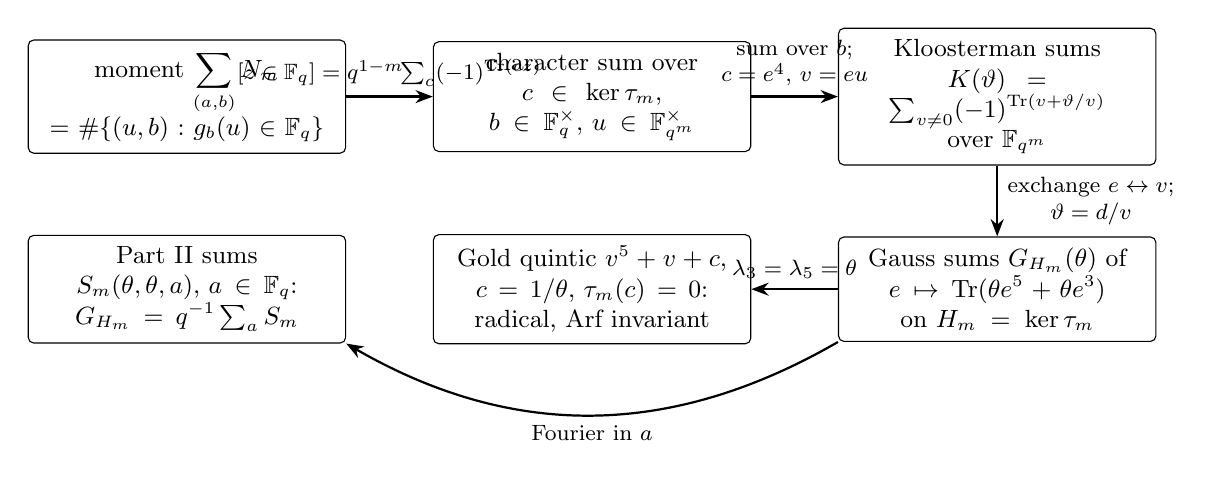
\begin{tikzpicture}[
  box/.style={draw,rounded corners=2pt,align=center,inner sep=4pt,font=\small,minimum height=1.1cm,text width=3.75cm},
  arr/.style={-{Stealth[length=2.2mm]},thick},
  lab/.style={font=\footnotesize,align=center,midway}
]
\node[box] (A) {moment $\displaystyle\sum_{(a,b)}N_m$\\ $=\#\{(u,b):g_b(u)\in\F_q\}$};
\node[box,right=1.1cm of A] (B) {character sum over\\ $c\in\ker\tau_m$, $b\in\F_q^\times$, $u\in\F_{q^m}^\times$};
\node[box,right=1.1cm of B] (C) {Kloosterman sums\\ $K(\vartheta)=\sum_{v\ne0}(-1)^{\Tr(v+\vartheta/v)}$\\ over $\F_{q^m}$};
\node[box,below=0.9cm of C] (D) {Gauss sums $G_{H_m}(\theta)$ of\\ $e\mapsto\Tr(\theta e^5+\theta e^3)$\\ on $H_m=\ker\tau_m$};
\node[box,left=1.1cm of D] (E) {Gold quintic $v^5+v+c$,\\ $c=1/\theta$, $\tau_m(c)=0$:\\ radical, Arf invariant};
\node[box,left=1.1cm of E] (F) {Part~II sums\\ $S_m(\theta,\theta,a)$, $a\in\F_q$:\\ $G_{H_m}=q^{-1}\sum_aS_m$};
\draw[arr] (A) -- node[lab,above]{$[z\in\F_q]=q^{1-m}\!\!\sum_{c}(-1)^{\Tr(cz)}$} (B);
\draw[arr] (B) -- node[lab,above]{sum over $b$;\\ $c=e^4$, $v=eu$} (C);
\draw[arr] (C) -- node[lab,right]{exchange $e\leftrightarrow v$;\\ $\vartheta=d/v$} (D);
\draw[arr] (D) -- node[lab,above]{$\lambda_3=\lambda_5=\theta$} (E);
\draw[arr] (D.south west) to[out=-150,in=-30] node[lab,below]{Fourier in $a$} (F.south east);
\end{tikzpicture}
\caption{The evaluation of the moments $\sum N_m$ (Propositions~\ref{prop:N3}, \ref{prop:Nm}): every step is an exact identity; the only quantities that are not elementary are the Gauss sums $G_{H_m}(\theta)$, which are $0$ or $\pm2^{(mk+r)/2}$ with $r$ the dimension of the radical on the hyperplane. No archimedean estimate enters anywhere, which is why the moments can be exact polynomials in $q$.}\label{fig:reduction}
\end{figure}

\subsection{The third moment}
Let $\Tr=\Tr_{q^3/2}$, $\tau=\Tr_{q^3/q}$, $H=\ker\tau\subset\F_{q^3}$ (an $\F_2$-space of dimension $2k$), and for $\theta\in\F_{q^3}$ put
\[
G_H(\theta)=\sum_{e\in H}(-1)^{\Tr(\theta e^5+\theta e^3)},\qquad \Theta=\{\theta\in\F_{q^3}^\times:\tau(\theta^{-1})=0\}.
\]
$G_H(\theta)$ is the Gauss sum of the $\F_2$-quadratic form $Q_\theta(e)=\Tr(\theta e^5+\theta e^3)$ (both exponents are of Gold type $2^i+1$; the polynomials $v^{2^i+1}+v+c$ are those of Bluher \cite{Bluher} and Helleseth--Kholosha \cite{HellesethKholosha}) restricted to the hyperplane $H$; equivalently $G_H(\theta)=q^{-1}\sum_{a\in\F_q}S_3(\theta,\theta,a)$ with $S_3(\lambda_5,\lambda_3,\lambda_1)=\sum_{e\in\F_{q^3}}(-1)^{\Tr(\lambda_5e^5+\lambda_3e^3+\lambda_1e)}$ the sums of Part~II over $\F_{q^3}$ (the curves $y^2+y=\lambda_5x^5+\lambda_3x^3$ are supersingular, cf.\ van der Geer--van der Vlugt \cite{vdGvdV}).

\begin{proposition}\label{prop:N3}
For every $q=2^k$,
\[
\sum_{(a,b)\in\F_q\times\F_q^\times}N_3(a,b)=(q-1)^2+\frac1q\sum_{\theta\in\Theta}G_H(\theta).
\]
\end{proposition}
\begin{proof}
By \eqref{eq:a}, $\sum N_3=\#\{(u,b)\in\F_{q^3}^\times\times\F_q^\times:g_b(u)\in\F_q\}$. The annihilator of $\F_q$ for the pairing $(c,z)\mapsto\Tr(cz)$ on $\F_{q^3}$ is $A=\{c:\tau(c)=0\}$, of order $q^2$, so $[z\in\F_q]=q^{-2}\sum_{c\in A}(-1)^{\Tr(cz)}$ and
\[
\sum N_3=\frac1{q^2}\sum_{c\in A}\sum_{b\in\F_q^\times}\sum_{u\ne0}(-1)^{\Tr(cu^4+cb/u+cb^2/u^2)}=\frac1{q^2}\sum_{c\in A}\sum_{b}\sum_{u}(-1)^{\Tr(c^{1/4}u)+\Tr(b(c+c^{1/2})/u)},
\]
using $\Tr(z^4)=\Tr(z^2)=\Tr(z)$. The sum over $b\in\F_q^\times$ is $q[\tau((c+c^{1/2})/u)=0]-1$. The part with $-1$ contributes $-q^{-2}\sum_{c\in A}\sum_{u\ne0}(-1)^{\Tr(c^{1/4}u)}=-q^{-2}\bigl((q^3-1)-(q^2-1)\bigr)=-(q-1)$. In the other part the term $c=0$ contributes $(q^3-1)/q$; for $c\ne0$ write $c=e^4$ with $e\in A\setminus0$ and substitute $v=eu$: the condition becomes $\tau((e^5+e^3)/v)=0$ and the weight $(-1)^{\Tr v}$, so this part equals
\[
\frac{q^3-1}q+\frac1{q^2}\sum_{e\in A\setminus0}\ \sum_{d\in\F_q}K\bigl(d(e^5+e^3)\bigr),\qquad K(\vartheta)=\sum_{v\ne0}(-1)^{\Tr(v+\vartheta/v)}
\]
(Kloosterman sums over $\F_{q^3}$, cf.\ Carlitz \cite{Carlitz} and Lachaud--Wolfmann \cite{LachaudWolfmann} for their arithmetic in characteristic $2$). The terms $d=0$ give $-(q^2-1)/q^2$. For $d\ne0$ we exchange the order: $\sum_{e\in A\setminus0}(-1)^{\Tr(d(e^5+e^3)/v)}=G_H(d/v)-1$, and with $\vartheta=d/v$,
\[
\sum_{d\ne0}\sum_{v\ne0}(-1)^{\Tr v}\bigl(G_H(d/v)-1\bigr)=(q-1)+\sum_{\vartheta\ne0}G_H(\vartheta)\bigl(q[\tau(\vartheta^{-1})=0]-1\bigr).
\]
Finally $\sum_{\vartheta\ne0}G_H(\vartheta)=q^3\#\{e\in H:e^5+e^3=0\}-|H|=q^3-q^2$, since $e^5+e^3=e^3(e+1)^2$ vanishes only at $e\in\{0,1\}$ and $1\notin H$ ($\tau(1)=3=1$). Collecting,
\begin{align*}
\sum N_3&=-(q-1)+\frac{q^3-1}q-\frac{q^2-1}{q^2}+\frac{(q-1)-(q^3-q^2)}{q^2}+\frac1q\sum_{\theta\in\Theta}G_H(\theta)\\
&=(q-1)^2+\frac1q\sum_{\theta\in\Theta}G_H(\theta).\qedhere
\end{align*}
\end{proof}

\begin{proposition}[structure of $G_H(\theta)$; numerical at $q=8,32,128$]\label{prop:GHstructure}
Let $\theta\in\Theta$ and $c=\theta^{-1}$ (so $\tau(c)=0$), and let (\texttt{moment3\_structure.py})
\[
R=\ker T_\theta\cap\F_{q^3},\qquad R_H=\{e\in H:T_\theta(e)\in\F_q\}
\]
be the radical of $Q_\theta$ on $\F_{q^3}$ (the $\sigma^3$-fixed part of the quintic frame of $v^5+v+c$, of dimension $1$ for the Gold types $(1,4)$, $(2,3)$ and $3$ for $(1,1,1,2)$) and the radical of the restriction $Q_\theta|_H$ (the orthogonal of $H$ for the absolute trace pairing is $\F_q$). For all $\theta\in\Theta$ at $q=8$, $32$ and $128$:
\begin{enumerate}[label=\textup{(\roman*)},leftmargin=2em]
\item $\dim R_H=2$, whatever the Gold type and $\dim R$;
\item $G_H(\theta)\ne0$ iff $Q_\theta$ vanishes on $R_H$;
\item whenever $G_H(\theta)\ne0$ the induced nondegenerate form on $H/R_H$ ($\dim 2k-2$) has Arf invariant $0$ \cite{Arf}, so $G_H(\theta)=+2^{k+1}$;
\item the joint distribution of the Gold type of $v^5+v+c$ over $\F_{q^3}$ and of the vanishing of $Q_\theta|_{R_H}$ is
\[
\begin{array}{l|cc|cc|cc}
 & \multicolumn{2}{c|}{(1,4)} & \multicolumn{2}{c|}{(2,3)} & \multicolumn{2}{c}{(1,1,1,2)}\\
 & G_H\ne0 & G_H=0 & G_H\ne0 & G_H=0 & G_H\ne0 & G_H=0\\
\hline
q=8 & 27 & 27 & 0 & 9 & 0 & 0\\
q=32 & 285 & 255 & 90 & 243 & 120 & 30\\
q=128 & 4347 & 4095 & 2436 & 2901 & 1344 & 1260
\end{array}
\]
with totals $27$, $495$, $8127$ of nonzero values, i.e.\ $(q+1)(q-2)/2$ in each case.
\end{enumerate}
\end{proposition}

\begin{remark}
The per-type counts $(54,9,0)$, $(540,333,150)$, $(2604,\dots)$ are not the values of a common quadratic polynomial with small denominators (the interpolating quadratics have coefficients like $331/640$; \texttt{part4\_moment\_system.py}), whereas the total number of $\theta$ with $G_H(\theta)\ne0$ is the clean polynomial $(q+1)(q-2)/2$. A proof of Conjecture~\ref{conj:N3value} must therefore count the vanishing locus of $Q_\theta|_{R_H}$ directly rather than type by type.
\end{remark}

\begin{conjecture}[verified for $q=8,32,128$; \texttt{moment3\_check.py}]\label{conj:N3value}
For odd $k$ the four statements of Proposition~\ref{prop:GHstructure} hold for every $q$; in particular $G_H(\theta)\in\{0,2^{k+1}\}$ and $\#\{\theta\in\Theta:G_H(\theta)\ne0\}=(q+1)(q-2)/2$. Consequently
\[
\sum_{(a,b)}N_3(a,b)=(q-1)^2+(q+1)(q-2)=2q^2-3q-1 ,
\]
which is the value predicted by Target Theorem~\ref{tgt:counts} (Proposition~\ref{prop:elimination}). At $q=8$: $103=49+54$; at $q=32$: $1951=961+990$; at $q=128$: $32383=16129+16254$.
\end{conjecture}

\begin{remark}[what a proof requires]
Because $\theta\in\F_{q^3}\setminus\F_q$, the operator $T_\theta$ does \emph{not} commute with $\sigma$, and the description of $\{e:T_\theta(e)\in\F_q\}$ through $(\sigma-1)^{-1}(\ker T_\theta)$ that drives Part~II (where the parameters lie in $\F_q$) is not available; this is why $\dim R_H=2$ although $\dim R=1$. Three facts are needed: (a) a description of the two-dimensional radical $R_H$, uniform in the Gold type; (b) the condition ``$Q_\theta|_{R_H}=0$'' as an explicit condition on $c$ and the count $(q+1)(q-2)/2$ of the $c\in\ker\tau$ satisfying it; (c) the vanishing of the Arf invariant. Through $G_H(\theta)=q^{-1}\sum_aS_3(\theta,\theta,a)$, (c) is a sign pattern of the Part~II sums along $a\in\F_q$, which the shift calculus of Part~II (with $c\in\F_{q^3}$, $T_\theta(c)\in\F_q$) should determine as in Part~II, Theorem~6.12. With $(\lambda_3,\lambda_5)=(\theta,\theta)$ the Bluher quintic of Part~II is $\theta(\theta u^5+\theta u+1)$, i.e.\ the Gold quintic $v^5+v+c$ with $c=\theta^{-1}$ and no scaling, so the condition $\theta\in\Theta$ is exactly the trace condition $\tau(c)=0$ on the Gold parameter; Part~II, Proposition~6.8 answers the analogous question over $\F_q$ (there $(q-2)/2$ Gold parameters are of type $(1,4)$), and the present question concerns the quintic over the cubic extension with a trace constraint.
\end{remark}

\subsection{All moments}
\begin{proposition}\label{prop:Nm}
For every $m\ge1$, with $\tau_m=\Tr_{q^m/q}$, $H_m=\ker\tau_m$, $\Theta_m=\{\theta\in\F_{q^m}^\times:\tau_m(\theta^{-1})=0\}$ and $G_{H_m}(\theta)=\sum_{e\in H_m}(-1)^{\Tr_{q^m/2}(\theta e^5+\theta e^3)}$,
\[
\sum_{(a,b)}N_m(a,b)=(q-1)^2-q\,[2\mid m]+q^{2-m}\sum_{\theta\in\Theta_m}G_{H_m}(\theta).
\]
\end{proposition}
\begin{proof}
The proof of Proposition~\ref{prop:N3} goes through with $3$ replaced by $m$: $|A|=q^{m-1}$, the part with $-1$ gives $-(q-1)$, the term $c=0$ gives $q^{2-m}(q^m-1)$, the terms $d=0$ give $-q^{1-m}(q^{m-1}-1)$, the terms $d\ne0$ give $q^{1-m}\bigl[(q-1)+q\sum_{\Theta_m}G_{H_m}-\sum_{\vartheta\ne0}G_{H_m}(\vartheta)\bigr]$ with $\sum_{\vartheta\ne0}G_{H_m}(\vartheta)=q^m\#\{e\in H_m:e^5+e^3=0\}-q^{m-1}$, and $\#\{e\in H_m:e^3(e+1)^2=0\}=1+[2\mid m]$ because $1\in H_m$ iff $\tau_m(1)=m$ vanishes in $\F_2$. Collecting the constants gives $(q-1)^2-q[2\mid m]$.
\end{proof}

\begin{remark}[consistency with Part~III, Theorem~1.3]\label{rem:m12}
For $m=1$: $\tau_1=\mathrm{id}$, so $\Theta_1=\varnothing$ and $\sum N_1=(q-1)^2$. For $m=2$: $H_2=\F_q$ and $\Theta_2=\F_q^\times$; for $\theta,e\in\F_q$ one has $\Tr_{q^2/2}(\theta(e^5+e^3))=\Tr_{q/2}(2\theta(e^5+e^3))=0$, hence $G_{H_2}(\theta)=q$ for every $\theta\in\Theta_2$ and
\[
\sum N_2=(q-1)^2-q+(q-1)q=2q^2-4q+1=(q-1)^2+q(q-2),
\]
which is $\sum N_1+\sum(N_2-N_1)$ with the values of Part~III, Theorem~1.3. Thus the two moments proved in Part~III by root counting are the cases in which the Gauss sums degenerate ($H_1=0$; $H_2=\F_q$ with the form identically zero), and $m=3$ is the first case in which the supersingular sums of Part~II genuinely enter.
\end{remark}

\subsection{The elimination system}
Let $n_C(q)$ be the class counts (mixed and pure pairs together) and $f^{(m)}_C$ the fixed-point numbers of Table~\ref{tab:classes}. Since $N_m(B_\lambda)=f^{(m)}_{C(\lambda)}$,
\begin{equation}\label{eq:moments}
\sum_{(a,b)}N_m=\sum_Cn_C(q)f^{(m)}_C,\qquad
\Sigma_m(q):=\sum_{\theta\in\Theta_m}G_{H_m}(\theta)=q^{m-2}\Bigl(\sum_{(a,b)}N_m-(q-1)^2+q[2\mid m]\Bigr).
\end{equation}

\begin{proposition}[\texttt{part4\_moment\_system.py}]\label{prop:elimination}
\begin{enumerate}[label=\textup{(\roman*)},leftmargin=2em]
\item The $6\times11$ matrix $(f^{(m)}_C)_{1\le m\le6}$ has rank $6$; the six moments $m\le6$ determine the eleven class counts up to a five-dimensional space. Adjoining the five mixed moments $\sum N_1N_2$, $\sum N_1N_3$, $\sum N_2^2$, $\sum N_1^2N_2$ and $\sum N_1N_2N_3$ raises the rank to $10$ only, whereas adjoining the five statistics
\begin{gather*}
M_{3,3}=\sum N_3^2,\qquad M_{2,3}=\sum N_2N_3,\qquad M_{2,2}=\sum N_2^2,\\
M_{1,3}=\sum N_1N_3,\qquad M_{3,3,3}=\sum N_3^3
\end{gather*}
gives an $11\times11$ matrix of determinant $1433272320=2^{17}\cdot3^7\cdot5\ne0$. Hence the eleven class counts are the unique solution of the linear system formed by the six pure moments and these five mixed moments, which are point counts on fibre products of the curves $C_m^{(b)}$ over the $a$-line (the two-fold products $C_3\times_{\mathbb A^1}C_3$, $C_2\times_{\mathbb A^1}C_3$, $C_2\times_{\mathbb A^1}C_2$, $C_1\times_{\mathbb A^1}C_3$ and the triple product of $C_3$). If the counts are those of Target Theorem~\ref{tgt:counts}, the five mixed moments are
\begin{gather*}
M_{3,3}=8q^2-12q-7,\qquad M_{2,3}=5q^2-11q+3,\qquad M_{2,2}=7q^2-18q+9,\\
M_{1,3}=3q^2-7q+3,\qquad M_{3,3,3}=38q^2-54q-43 ,
\end{gather*}
and back-substitution of these eleven values returns the table. Target Theorem~\ref{tgt:counts} is therefore equivalent to eleven explicit point counts: six on the curves $C_m^{(b)}$ and five on their fibre products.
\item If the counts are those of Target Theorem~\ref{tgt:counts}, then the moments and the Gauss-sum totals are
\[
\begin{array}{c|l|l}
m & \sum_{(a,b)}N_m & \Sigma_m=\sum_{\Theta_m}G_{H_m}\\
\hline
1 & (q-1)^2 & 0\\
2 & 2q^2-4q+1 & q(q-1)\\
3 & 2q^2-3q-1 & q(q+1)(q-2)\\
4 & 3q^2-6q+1 & q^3(2q-3)\\
5 & 2q^2-2q+2 & q^3(q^2+1)\\
6 & 4q^2-4q-1 & q^4(q-1)(3q+2)
\end{array}
\]
Conversely, Target Theorem~\ref{tgt:counts} is equivalent to these six evaluations together with the five mixed moments; the rows $m=1,2$ are theorems (Part~III), the row $m=3$ is Conjecture~\ref{conj:N3value}.
\end{enumerate}
\end{proposition}
\begin{proof}
(i) is a rank computation (the matrix is printed by the script). (ii) is the substitution of the table into \eqref{eq:moments}; the second column is then a direct consequence of Proposition~\ref{prop:Nm}. For the converse note that the class counts are integers determined by the eleven joint fixed-point statistics, which are linear combinations of the pure and mixed moments.
\end{proof}

\begin{remark}
The rows are a list of exact Gauss-sum identities to be proved. The row $m=4$ reads $\sum_{\theta\in\F_{q^4}^\times,\ \tau_4(1/\theta)=0}G_{H_4}(\theta)=q^3(2q-3)$ with $H_4$ of dimension $3k$: the forms $e\mapsto\Tr_{q^4/2}(\theta e^5+\theta e^3)$ have radicals controlled by the Gold quintic over $\F_{q^4}$, whose factorisation types over $\F_{q^4}$ are those of Part~II, Proposition~6.8, extended by the splitting of $\F_{q^4}(\mu_5)$; the rows $m=5,6$ involve the Gold quintic over $\F_{q^5}$ and $\F_{q^6}$, where $\mu_5\subset\F_{q^4}$ enters for $m\equiv0\bmod4$ only. This is the precise sense in which the counts of Target Theorem~\ref{tgt:counts} are polynomial: each $\Sigma_m$ is a sum of terms $0,\pm2^{(mk+r)/2}$ whose number is a polynomial point count on the Gold-quintic curves over $\F_{q^m}$ with a trace constraint, and the Arf invariants are constant on the strata; there is no cuspidal cohomology to control because every sum involved is supersingular (all normalised Frobenius eigenvalues are roots of unity), which is the structural reason for the absence of $O(q^{1/2})$ error terms. Turning this into a proof means establishing (a)--(c) of the remark after Conjecture~\ref{conj:N3value} for each $m\le6$ and for the fibre products; the authors of \cite{KatzKR} reach polynomial answers in the odd-characteristic setting by Deligne's theory \cite{Deligne}, which here is replaced by the exact Witt-vector evaluation.
\end{remark}

\section{Explicit Brown invariants of length-two Witt sheaves}\label{sec:brown}

\subsection{The shift calculus and representative cosets}
Recall from Part~III (Lemma~6.4): for $c\in\F_{q^m}$ with $T'_\lambda(c)=a\in\F_q$,
\begin{equation}\label{eq:shift}
s_m(\lambda_1)=i^{\qq^{(m)}_\lambda(c)}\,s_m(\lambda_1+a)\qquad(\lambda_3,\lambda_5\text{ fixed}),
\end{equation}
which follows from \eqref{eq:polar} by substituting $x\mapsto x+c$. More generally, for any $c\in\F_{q^m}$ the same substitution gives $s_m(\lambda_1)=i^{\qq^{(m)}_\lambda(c)}\,s_m(\lambda_1+T'_\lambda(c))$ with $\lambda_1+T'_\lambda(c)\in\F_{q^m}$, where $s_m$ is extended to parameters $\lambda_1\in\F_{q^m}$ by the same formula.

\begin{lemma}\label{lem:coset}
Let $V^{(m)}_\lambda=\{c\in\F_{q^m}:T'_\lambda(c)\in\F_q\}$ and let $a_1,\dots,a_t$ be representatives of the cosets of $T'_\lambda(V^{(m)}_\lambda)$ in $\F_q$. Then $\lambda_1\mapsto s_m(\lambda_1)$ is determined by its values at $a_1,\dots,a_t$ together with the phases $\qq^{(m)}_\lambda(c)$, $c\in V^{(m)}_\lambda$; one element $c$ per coset of $\Kk_\lambda\cap\F_{q^m}$ in $V^{(m)}_\lambda$ suffices. In particular, for $m=4$ and $N_0\mid4$: $T'_\lambda(V^{(4)}_\lambda)=\F_q$ unless $N_0=4$, where it is the hyperplane $\tau_0^\perp$; a single value and the phases decide all of $\lambda_1\mapsto s_4(\lambda_1)$.
\end{lemma}
\begin{proof}
Immediate from \eqref{eq:shift}; the image statements are Part~III, Proposition~6.15(i).
\end{proof}

Two general facts about the Gauss sums will be used repeatedly. Let $R_m=\Kk_\lambda\cap\F_{q^m}=\Kk_\lambda^{\sigma^m}$, the radical of the polar form of $\qq^{(m)}_\lambda$ on $\F_{q^m}$ (by \eqref{eq:polar} and the nondegeneracy of the trace pairing), of dimension $f_m$.

\begin{lemma}\label{lem:gaussbasics}
\begin{enumerate}[label=\textup{(\roman*)},leftmargin=2em]
\item $\qq^{(m)}_\lambda$ is additive on $R_m$, and $s_m(\lambda)\ne0$ iff $\qq^{(m)}_\lambda$ vanishes on $R_m$; in that case $|s_m(\lambda)|^2=2^{mk+f_m}$.
\item $\qq^{(m)}_{\lambda_1+1}(x)=\qq^{(m)}_{\lambda_1}(x)+2\Tr_{q^m/2}(x)$ and $\qq^{(m)}_\lambda(x)\equiv\Tr_{q^m/2}(x)\pmod2$; consequently $s_m(\lambda_1+1)=\overline{s_m(\lambda_1)}$.
\item Write $s_m(\lambda)=\mathrm{Re}+i\,\mathrm{Im}$ with
\[
\mathrm{Re}=\sum_{\Tr x=0}(-1)^{\qq(x)/2},\qquad \mathrm{Im}=\sum_{\Tr x=1}(-1)^{(\qq(x)-1)/2}.
\]
These are Gauss sums of $\F_2$-valued quadratic forms on the hyperplane $\ker\Tr_{q^m/2}$ (the second one shifted by a constant), hence each lies in $\{0\}\cup\{\pm2^j:j\ge0\}$ \cite{LidlNiederreiter}.
\item There is $\lambda_1'\in\F_q$ with $s_m(\lambda_1')\ne0$ if and only if $\frac12\qq^{(m)}_{\lambda,\lambda_1=0}$ vanishes on $R_m\cap\ker\tau_m$. This holds for $m=1$.
\end{enumerate}
\end{lemma}
\begin{proof}
(i) Additivity on $R_m$ is \eqref{eq:polar}. If $\qq(\kappa)\ne0$ for some $\kappa\in R_m$, the substitution $x\mapsto x+\kappa$ multiplies $s_m$ by $i^{\qq(\kappa)}\ne1$, so $s_m=0$. Otherwise $|s_m|^2=\sum_{x,z}i^{\qq(x+z)-\qq(x)}=\sum_zi^{\qq(z)}\sum_x(-1)^{\Tr(xT'(z))}=q^m\sum_{z\in R_m}i^{\qq(z)}=q^m|R_m|$. (ii) The first identity is the definition, the congruence is $\Tw_{mk}\equiv\Tr\bmod2$; the terms with $\Tr x=0$ are real and unchanged under $\lambda_1\mapsto\lambda_1+1$, those with $\Tr x=1$ are purely imaginary and change sign. (iii) On $H_0=\ker\Tr$ the values of $\qq$ are even and $Q_0=\qq/2$ satisfies $Q_0(x+y)=Q_0(x)+Q_0(y)+\Tr(yT'(x))$ by \eqref{eq:polar}, a quadratic form; on $x_1+H_0$ one has $(\qq(x_1+h)-1)/2=(\qq(x_1)-1)/2+Q_0(h)+\Tr(hT'(x_1))$. Gauss sums of $\F_2$-quadratic forms are $0$ or $\pm2^{(\dim+\mathrm{rad})/2}$. (iv) By (i), $s_m(\lambda_1)\ne0$ iff $\qq_0(\kappa)+2\Tr_{q/2}(\lambda_1\tau_m(\kappa))=0$ for all $\kappa\in R_m$, i.e.\ iff the linear functional $\frac12\qq_0$ on $R_m$ equals $\kappa\mapsto\Tr_{q/2}(\lambda_1\tau_m(\kappa))$; such a $\lambda_1$ exists iff $\frac12\qq_0$ factors through $\tau_m|_{R_m}$, every linear functional on the subspace $\tau_m(R_m)\subset\F_q$ being of the form $\Tr_{q/2}(\lambda_1\,\cdot)$. For $m=1$, $\tau_1$ is the identity.
\end{proof}

\subsection{The hexad formula}
\begin{theorem}[hexad formula]\label{thm:hexadformula}
Let $\lambda_5\ne0$, $m\ge1$, and let $\eps(w)=+1$ if $B_\lambda(w)=0$ and $\eps(w)=-1$ otherwise. Then
\begin{equation}\label{eq:hexadformula}
s_{2m}(\lambda)=q^m\sum_{w\in T_\lambda'^{-1}(1)\cap\F_{q^m}}\eps(w)\,i^{\qq^{(m)}_\lambda(w)} .
\end{equation}
Here $T_\lambda'^{-1}(1)=r_1+\Kk_\lambda$ consists of the six roots of $B_\lambda$ and the ten synthematic totals, so the sum has at most sixteen terms; the set $T_\lambda'^{-1}(1)\cap\F_{q^m}$ is $r+\Kk_\lambda^{\sigma^m}$ for any $r\in T_\lambda'^{-1}(1)\cap\F_{q^m}$, and is empty if there is no such $r$.
\end{theorem}
\begin{proof}
Write $V=\F_{q^{2m}}$, $U=\F_{q^m}$, $\qq=\qq^{(2m)}_\lambda$, $\Tr=\Tr_{q^{2m}/2}$, $\varphi=\sigma^m$ (so $\varphi(x)=x^{q^m}$ and $\Tr_{q^{2m}/q^m}=\varphi+1$).

\emph{Step 1: $\qq$ on $U$.} For $u\in U$, $\Tw_{2mk}(u)=\Tr_{W_2(U)/\Z/4}([u]+[u])=\Tr_{W_2(U)/\Z/4}(0,u^2)=2\Tr_{q^m/2}(u)$ and $2\Tr(f(u))=4\Tr_{q^m/2}(f(u))=0$; so $\qq(u)=2\Tr_{q^m/2}(u)$.

\emph{Step 2: summation over the cosets of $U$.} For $c\in V$, $u\in U$, by \eqref{eq:polar} and Step 1,
\[
\qq(c+u)=\qq(c)+2\Tr_{q^m/2}(u)+2\Tr\bigl(uT'(c)\bigr)=\qq(c)+2\Tr_{q^m/2}\bigl(u\,(1+(\varphi+1)T'(c))\bigr),
\]
hence $\sum_{u\in U}i^{\qq(c+u)}=i^{\qq(c)}\,q^m\,[(\varphi+1)T'(c)=1]$, and $\qq$ is constant on the cosets $c+U$ with $(\varphi+1)T'(c)=1$ (this condition depends only on the coset, since $T'(U)\subset U=\ker(\varphi+1)$). Therefore
\[
s_{2m}(\lambda)=\sum_{c\in V/U}\sum_{u\in U}i^{\qq(c+u)}=q^m\sum_{\substack{c\in V/U\\ (\varphi+1)T'(c)=1}}i^{\qq(c)} .
\]
Since $T'$ has coefficients in $\F_q$ it commutes with $\varphi$, so $(\varphi+1)T'(c)=T'((\varphi+1)c)$, and the condition reads $w:=c+c^{q^m}\in T'^{-1}(1)$. As $\varphi+1$ maps $V$ onto $U$ with kernel $U$, the cosets $c+U$ correspond bijectively to the elements $w\in U$, and $w\in T'^{-1}(1)\cap U$. It remains to show $\qq(c)=\qq^{(m)}_\lambda(w)+2[\eps(w)=-1]$ for any $c$ with $c+c^{q^m}=w$.

\emph{Step 3: the Witt value of $c$.} Let $N=c\,c^{q^m}\in U$. By transitivity of the trace of Witt vectors and $\varphi([c])=[c^{q^m}]$,
\[
\Tw_{2mk}(c)=\Tr_{W_2(U)/\Z/4}\bigl([c]+[c^{q^m}]\bigr)=\Tr_{W_2(U)/\Z/4}(w,N)=\Tw_{mk}(w)+2\Tr_{q^m/2}(N),
\]
using $[x]+[y]=(x+y,xy)$ in $W_2$ of a ring of characteristic $2$ and $(w,N)=[w]+V[N]$. The power sums $p_j=c^j+c^{jq^m}$ of the two conjugates are, by Newton's identities with $e_1=w$, $e_2=N$: $p_1=w$, $p_3=w^3+Nw$, $p_5=w^5+Nw^3+N^2w$. Hence
\begin{align*}
\qq(c)&=\Tw_{mk}(w)+2\Tr_{q^m/2}\bigl(N+\lambda_5p_5+\lambda_3p_3+\lambda_1p_1\bigr)\\
&=\qq^{(m)}_\lambda(w)+2\Tr_{q^m/2}\bigl(N(1+\lambda_5w^3+\lambda_3w)+\lambda_5N^2w\bigr)=\qq^{(m)}_\lambda(w)+2\Tr_{q^m/2}(N\gamma_w),
\end{align*}
with $\gamma_w=1+\lambda_5w^3+\lambda_3w+(\lambda_5w)^{1/2}$ (as $\Tr(\lambda_5N^2w)=\Tr(N(\lambda_5w)^{1/2})$). Now $\gamma_w^2=1+\lambda_5^2w^6+\lambda_3^2w^2+\lambda_5w=B_\lambda(w)$, and from $T'(w)=1$, i.e.\ $\lambda_5w^4+\lambda_3w^2+w=1+(\lambda_3w)^{1/2}+(\lambda_5w)^{1/4}$,
\[
w\gamma_w=w+\lambda_5w^4+\lambda_3w^2+(\lambda_5w^3)^{1/2}=1+(\lambda_3w)^{1/2}+(\lambda_5w)^{1/4}+(\lambda_5w^3)^{1/2},\qquad (w\gamma_w)^2=\gamma_w .
\]
So $\gamma_w\in\{0,w^{-2}\}$ ($w\ne0$ since $T'(0)=0$), and $\gamma_w=0$ iff $B_\lambda(w)=0$. If $w$ is a root, $\qq(c)=\qq^{(m)}_\lambda(w)$. If $w$ is a total, $N\gamma_w=(c^2+cw)/w^2=v^2+v$ with $v=c/w$, and $v+v^{q^m}=1$, so $v\notin U$ and the Artin--Schreier polynomial $Y^2+Y+(v^2+v)$ over $U$ has no root in $U$, i.e.\ $\Tr_{q^m/2}(v^2+v)=1$; thus $\qq(c)=\qq^{(m)}_\lambda(w)+2$. This is the claim, and \eqref{eq:hexadformula} follows. The description of $T'^{-1}(1)$ is Part~III, Theorem~1.1 and \S4.
\end{proof}

\begin{remark}
(1) For $N_0\mid4$ the formula with $m=2$ makes $s_4$, a sum over $q^4$ elements, a sum of $4$ (classes of order $4$) or $16$ (classes with $N_0\mid2$) terms $\pm i^{\qq^{(2)}(w)}$ times $q^2$; for $N_0\in\{3,6\}$, $m=3$ gives $s_6$ as $q^3$ times $16$ (classes $3\,1^3$, $3^2$), $8$ ($3\,2\,1$) or $4$ (class $6$) terms. Table~\ref{tab:hexadterms} lists the patterns at $q=8$. (2) Equivalently: $s_{2m}=\sum_{c\in A}i^{\qq(c)}$ over the affine space $A=\{c\in\F_{q^{2m}}:\Tr_{q^{2m}/q^m}T'(c)=1\}$, a union of $|T'^{-1}(1)\cap\F_{q^m}|$ cosets of $\F_{q^m}$ on each of which $\qq$ is constant; in the classes of order $4$, $|A|=4q^2$ and $s_4\ne0$ iff $\qq$ is constant on $A$ (\texttt{part4\_relative\_reduction.py}, verified $q=8$ all pairs, $q=32$ four pairs per class). (3) Formula \eqref{eq:hexadformula} does not use the values $s_4\in\{0,\pm4q^2\}$ of Part~III; in the classes of order $4$ it reproves them (Theorem~\ref{thm:order4}).
\end{remark}

\begin{table}[htbp]
\centering
\caption{The signed terms $(\eps(w),\qq^{(m)}_\lambda(w))$ of the hexad formula at $q=8$, all $(\lambda_3,\lambda_5,\lambda_1)$ of each class (\texttt{part4\_hexad\_formula.py}); ``$a{:}b$'' means $a$ roots and $b$ totals with the given Witt value. The last column is $s_{2m}/q^m$.}\label{tab:hexadterms}
\small
\begin{tabular}{@{}llllr@{}}
\toprule
class & $m$ & roots: values & totals: values & $s_{2m}/q^m$\\
\midrule
$2^21^2$ & 2 & $2{:}0,\ 4{:}2$ & $6{:}0,\ 4{:}2$ & $-4$ (12 triples)\\
         &   & $4{:}0,\ 2{:}2$ & $4{:}0,\ 6{:}2$ & $+4$ (6)\\
         &   & $6{:}2$ & $10{:}2$ & $+4$ (6)\\
$2^3$    & 2 & $4{:}0,\ 2{:}2$ & $4{:}0,\ 6{:}2$ & $+4$ (6)\\
         &   & $6{:}2$ & $10{:}2$ & $+4$ (2)\\
$4\,1^2$ & 2 & $2{:}0$ & $2{:}2$ & $+4$ (24)\\
         &   & $2{:}0$ & $2{:}0$ & $0$ (24)\\
$4\,2$   & 2 & $2{:}2$ & $2{:}0$ & $-4$ (24)\\
         &   & $2{:}0$ & $2{:}0$ & $0$ (24)\\
$3\,1^3$ & 3 & $6{:}1$ & $10{:}1$ & $-4i$ (3)\\
         &   & $2{:}1,\ 4{:}3$ & $6{:}1,\ 4{:}3$ & $-4i$ (9)\\
         &   & $4{:}1,\ 2{:}3$ & $4{:}1,\ 6{:}3$ & $+4i$ (9)\\
         &   & $6{:}3$ & $10{:}3$ & $+4i$ (3)\\
$3^2$    & 3 & $6{:}1$ & $10{:}1$ & $-4i$ (12)\\
         &   & $6{:}3$ & $10{:}3$ & $+4i$ (12)\\
$3\,2\,1$& 3 & $1{:}0,\ 3{:}2$ & $3{:}0,\ 1{:}2$ & $-4$ (18)\\
         &   & $3{:}0,\ 1{:}2$ & $1{:}0,\ 3{:}2$ & $+4$ (18)\\
         &   & $4{:}0$ or $4{:}2$ & $4{:}0$ or $4{:}2$ & $0$ (36)\\
$6$      & 3 & --- & $4{:}1$ & $-4i$ (48)\\
         &   & --- & $4{:}3$ & $+4i$ (48)\\
\bottomrule
\end{tabular}
\end{table}

\subsection{Trace parity on the hexad coset}
\begin{theorem}[trace parity]\label{thm:traceparity}
Let $\lambda_5\ne0$, $m\ge1$, $w\in T_\lambda'^{-1}(1)\cap\F_{q^m}$, and suppose $s_m(\lambda_1')\ne0$ for some $\lambda_1'\in\F_q$ (Lemma~\ref{lem:gaussbasics}(iv)). Then
\[
\Tr_{q^m/2}(w)\equiv mk+f_m\pmod 2,\qquad f_m=\dim_{\F_2}\Kk_\lambda^{\sigma^m}.
\]
In particular all elements of $T_\lambda'^{-1}(1)\cap\F_{q^m}$, roots and totals alike, have the same absolute trace.
\end{theorem}
\begin{proof}
Put $s=s_m(\lambda_1')\ne0$ and $\qq=\qq^{(m)}_{\lambda,\lambda_1'}$. The shift identity with $c=w$, $T'(w)=1$, and Lemma~\ref{lem:gaussbasics}(ii) give
\[
s=i^{\qq(w)}\,s_m(\lambda_1'+1)=i^{\qq(w)}\,\bar s .
\]
By Lemma~\ref{lem:gaussbasics}(i),(iii), $s=\mathrm{Re}+i\,\mathrm{Im}$ with $\mathrm{Re}^2+\mathrm{Im}^2=2^{mk+f_m}$ and $\mathrm{Re},\mathrm{Im}\in\{0,\pm2^j\}$. If $mk+f_m$ is even, a power of $4$ is a sum of two squares of this shape only if one of them is $0$: $s$ is real or purely imaginary, $\bar s=\pm s$, so $i^{\qq(w)}=\pm1$, $\qq(w)$ is even and $\Tr_{q^m/2}(w)\equiv\qq(w)\equiv0$. If $mk+f_m$ is odd, then $\mathrm{Re}^2=\mathrm{Im}^2=2^{mk+f_m-1}$, so $s/\bar s=(\mathrm{Re}+i\,\mathrm{Im})^2/(\mathrm{Re}^2+\mathrm{Im}^2)=\pm i$, $\qq(w)$ is odd and $\Tr_{q^m/2}(w)=1$.
\end{proof}

\begin{corollary}[rational roots]\label{cor:rationalroots}
Let $k$ be odd and $r\in\F_q$ a root of $B_\lambda$ (equivalently of $F_{a,b}$) of class $C$. Then $\Tr_{q/2}(r)\equiv f_1(C)+1\pmod2$: the rational roots have trace $0$ in the classes $2\,1^4$, $3\,2\,1$, $4\,1^2$ and trace $1$ in the classes $1^6$, $2^21^2$, $3\,1^3$, $5\,1$. The same holds for the rational synthematic totals. For even $k$ the trace is $f_1(C)\bmod2$.
\end{corollary}
\begin{proof}
$m=1$ in Theorem~\ref{thm:traceparity}, the hypothesis being automatic by Lemma~\ref{lem:gaussbasics}(iv); $f_1$ is read off Table~\ref{tab:classes}.
\end{proof}

\begin{remark}
(1) The corollary is verified for every $(a,b)$ and every rational root at $q=8,32,128$ (\texttt{part4\_trace\_parity.py}: e.g.\ at $q=128$ the $4032$ rational roots of the class $4\,1^2$ all have trace $0$ and the $3277$ of the class $5\,1$ all have trace $1$). It is compatible with, and sharper than, the pair lemma of Part~III ($\Tr(r+s)=0$ for two rational roots), which it explains: two rational roots of one sextic lie in the same class. It is also compatible with $\sum N_1=(q-1)^2$: rational roots of both traces exist in abundance, distributed over the classes according to the parity of $f_1$. (2) For $m=2$ in the classes of order $4$, $R_2=\{0,r_1+r_3,r_2+r_4,\tau_0\}$, $\tau_2(r_1+r_3)=\tau_0\ne0$ and $\tau_2(\tau_0)=0$, so $R_2\cap\ker\tau_2=\{0,\tau_0\}$ and the hypothesis holds because $\qq^{(2)}(\tau_0)=2\Tr_{q/2}(\tau_0)=0$ (pair lemma); the conclusion $\Tr_{q^2/2}(w)=0$ for the four elements of $T'^{-1}(1)\cap\F_{q^2}$ is visible in Table~\ref{tab:hexadterms}. For $m=3$ in the classes $3^2$ and $6$, $\tau_3$ vanishes identically on $R_3$, so the hypothesis is the nonvanishing of $s_3$ for \emph{some} (equivalently every) $\lambda_1$; see \S\ref{subsec:N0div6}.
\end{remark}

\subsection{The classes of order 4}\label{subsec:order4}
Let $B_\lambda$ have class $4\,1^2$ or $4\,2$, with $4$-cycle $(r_1r_2r_3r_4)$, remaining roots $r_5,r_6$, $\tau_0=r_5+r_6\in\F_q^\times$, $\rho_0=r_5r_6\in\F_q$. The quadratic $u^2+\tau_0u+\rho_0$ splits over $\F_q$ iff $\Tr_{q/2}(\rho_0/\tau_0^2)=0$ iff the class is $4\,1^2$ (substitute $u=\tau_0y$). Since $r_1+r_2+r_3+r_4=\tau_0$ (the six roots sum to $0$),
\begin{gather*}
\Kk_\lambda^{\sigma^2}=\{0,\ r_1+r_3,\ r_2+r_4,\ \tau_0\},\qquad T_\lambda'^{-1}(1)\cap\F_{q^2}=\{r_5,\ r_6,\ w_3,\ w_4\},\\
w_3=r_5+r_1+r_3,\qquad w_4=r_5+r_2+r_4=w_3+\tau_0 ;
\end{gather*}
$w_3,w_4$ are the two synthematic totals of the synthemes $\{13|24|56\}$ (they are not roots: $w_3=r_j$ would force two roots to coincide). In the class $4\,2$, $\sigma(w_3)=r_6+r_2+r_4=w_3$, so $w_3,w_4\in\F_q$; in the class $4\,1^2$, $\sigma(w_3)=w_4$, so $w_3,w_4\in\F_{q^2}\setminus\F_q$ are conjugate with $w_3+w_4=\tau_0$.

\begin{lemma}[the roots outside the $4$-cycle]\label{lem:r5}
For every $\lambda_1$: $\qq^{(2)}_\lambda(\tau_0)=0$, $\qq^{(2)}_\lambda(r_6)=\qq^{(2)}_\lambda(r_5)$, $\qq^{(2)}_\lambda(w_4)=\qq^{(2)}_\lambda(w_3)$, and all four values $\qq^{(2)}_\lambda(r_5)$, $\qq^{(2)}_\lambda(r_6)$, $\qq^{(2)}_\lambda(w_3)$, $\qq^{(2)}_\lambda(w_4)$ are even. Moreover $\qq^{(4)}_\lambda(r_5)=\qq^{(4)}_\lambda(r_6)=\qq^{(4)}_\lambda(\tau_0)=0$.
\end{lemma}
\begin{proof}
$\tau_0\in\F_q$, so $\qq^{(2)}_\lambda(\tau_0)=\Tw_{2k}(\tau_0)+2\Tr_{q^2/2}(f(\tau_0))=2\Tr_{q/2}(\tau_0)+0=0$ by the pair lemma (Part~III, Theorem~1.3). For $x\in\{r_5,w_3\}$, $T'(x)=1$ and $\tau_0\in\Kk_\lambda$ give $\qq^{(2)}(x+\tau_0)=\qq^{(2)}(x)+\qq^{(2)}(\tau_0)+2\Tr_{q^2/2}(\tau_0)=\qq^{(2)}(x)$, which is the second and third claim (in the class $4\,2$ also $r_6=\sigma r_5$ and $\qq^{(2)}$ is $\sigma$-invariant). Parity: $\Tr_{q^2/2}(r_5)=\Tr_{q/2}(\tau_2(r_5))$ is $\Tr_{q/2}(\tau_0)=0$ or $\Tr_{q/2}(2r_5)=0$, and likewise for $w_3$ ($\tau_2(w_3)=\tau_0$ or $2w_3$). The last assertion is the multiplicity formula of Part~III, Lemma~6.5: $\qq^{(4)}_\lambda(x)=2\qq^{(2)}_\lambda(x)$ for $x\in\F_{q^2}$, and the three values of $\qq^{(2)}$ are even.
\end{proof}

\begin{theorem}[the classes of order $4$]\label{thm:order4}
Let $k$ be odd and $B_\lambda$ of class $4\,1^2$ or $4\,2$. For every $\lambda_1\in\F_q$:
\begin{enumerate}[label=\textup{(\roman*)},leftmargin=2em]
\item $s_4(\lambda_1)=2q^2\bigl(i^{\qq^{(2)}_\lambda(r_5)}-i^{\qq^{(2)}_\lambda(w_3)}\bigr)$, both exponents being even;
\item in the class $4\,1^2$: $\qq^{(2)}_\lambda(r_5)=0$ and $s_4(\lambda_1)=2q^2\bigl(1-(-1)^{\frac12\qq^{(2)}_\lambda(w_3)}\bigr)\in\{0,+4q^2\}$;
\item in the class $4\,2$: $\qq^{(2)}_\lambda(w_3)=0$ and $s_4(\lambda_1)=2q^2\bigl((-1)^{\frac12\qq^{(2)}_\lambda(r_5)}-1\bigr)\in\{0,-4q^2\}$;
\item consequently $\sgn s_4(\lambda_1)=(-1)^{\Tr_{q/2}(\rho_0/\tau_0^2)}$ whenever $s_4(\lambda_1)\ne0$; the set $\{\lambda_1:s_4(\lambda_1)\ne0\}$ is the affine hyperplane $\Tr_{q/2}(\lambda_1\tau_0)=\kappa_0$ with
\[
\kappa_0=1+\tfrac12\qq^{(2)}_{\lambda,\lambda_1=0}(w_3)\ \ (4\,1^2),\qquad \kappa_0=1+\tfrac12\qq^{(2)}_{\lambda,\lambda_1=0}(r_5)\ \ (4\,2);
\]
and $W'(\lambda_3,\lambda_5)=+2q^7$ in the class $4\,1^2$, $-2q^7$ in the class $4\,2$.
\end{enumerate}
\end{theorem}
\begin{proof}
(i) Theorem~\ref{thm:hexadformula} with $m=2$, the description of $T'^{-1}(1)\cap\F_{q^2}$ above, and Lemma~\ref{lem:r5}. (ii) In the class $4\,1^2$, $r_5\in\F_q$ is a root of class $4\,1^2$ with $f_1=1$, so $\Tr_{q/2}(r_5)=0$ by Corollary~\ref{cor:rationalroots}, and $\qq^{(2)}_\lambda(r_5)=\Tw_{2k}(r_5)+2\Tr_{q^2/2}(f_\lambda(r_5))=2\Tr_{q/2}(r_5)+0=0$. (iii) In the class $4\,2$, $w_3\in\F_q$ is a rational element of $T'^{-1}(1)$ of class $4\,2$ with $f_1=1$, so $\Tr_{q/2}(w_3)=0$ by Corollary~\ref{cor:rationalroots} (which applies to totals), and $\qq^{(2)}_\lambda(w_3)=2\Tr_{q/2}(w_3)=0$. (iv) The sign statement is (ii), (iii) and the splitting criterion. For the hyperplane, $\qq^{(2)}_\lambda(x)=\qq^{(2)}_{\lambda,0}(x)+2\Tr_{q^2/2}(\lambda_1x)=\qq^{(2)}_{\lambda,0}(x)+2\Tr_{q/2}(\lambda_1\tau_2(x))$ and $\tau_2(w_3)=\tau_0$ in the class $4\,1^2$, $\tau_2(r_5)=\tau_0$ in the class $4\,2$; so $s_4(\lambda_1)\ne0$ iff $\frac12\qq^{(2)}_{\lambda,0}(x)+\Tr_{q/2}(\lambda_1\tau_0)=1$ for $x=w_3$, resp.\ $r_5$. Finally $\Spp=q^4s_4$ (Part~III, Theorem~6.12) and the hyperplane has $q/2$ points, so $W'=\frac q2\cdot q^4\cdot(\pm4q^2)=\pm2q^7$.
\end{proof}

\begin{remark}
(1) Theorem~\ref{thm:order4} proves the order-$4$ part of Target Theorem~\ref{tgt:signs} and reproves Part~III, Theorem~6.12 and Corollary~6.13 in these classes without the $L$-polynomial argument. Numerically it is confirmed, with all $\lambda_1$, for all $12$ pairs at $q=8$ and all $240$ pairs at $q=32$ (\texttt{part4\_order4\_all.py}: sign, hyperplane $\Tr(\lambda_1\tau_0)=\kappa_0$ with $\kappa_0$ from \eqref{eq:q4r1} and \eqref{eq:kappaclosed}, and $W'=\pm2q^7$ on every pair); the values of $W'$ on the whole classes are also known for $q\le128$ from Part~II. (2) The two ingredients are of different nature: the hexad formula is an exact identity between Gauss sums over $\F_{q^4}$ and $\F_{q^2}$; the trace parity theorem is an \emph{arithmetic} statement about the rational points of the coset $T'^{-1}(1)$, proved by playing the shift identity against complex conjugation. The sign of the Brown invariant of $\qq^{(4)}_\lambda$ on $\F_{q^4}/\Kk_\lambda$ is thus $(-1)^{\Tr(\rho_0/\tau_0^2)}$ because the roots $r_5,r_6$ and the totals $w_3,w_4$ exchange their fields of definition between the two classes ($r_5\in\F_q$, $w_3\in\F_{q^2}\setminus\F_q$ in $4\,1^2$; $r_5\in\F_{q^2}\setminus\F_q$, $w_3\in\F_q$ in $4\,2$), while the rational one of the two always has trace $0$ and the sign $\eps$ distinguishes them. (3) The hyperplane parameter $\kappa_0$ of (iv) coincides with Part~III's $\kappa_0=\frac12\qq^{(4)}_{\lambda,0}(r_1+r_5)$, both describing the same set; Proposition~\ref{prop:kappa} gives it in closed form.
\end{remark}

\subsection{The hyperplane parameter and the quartic cofactor}
\begin{lemma}[the quartic cofactor]\label{lem:cofactor}
Write $B_\lambda/\lambda_5^2=u^6+au^2+bu+b^2$ with $a=\lambda_3^2/\lambda_5^2$, $b=\lambda_5^{-1}$, and let $u^2+\tau_0u+\rho_0$ be the quadratic factor with roots $r_5,r_6$. Then
\begin{gather*}
\frac{u^6+au^2+bu+b^2}{u^2+\tau_0u+\rho_0}=u^4+\tau_0u^3+(\tau_0^2+\rho_0)u^2+\tau_0^3u+\frac{b^2}{\rho_0},\\
\tau_0b^2+\rho_0b+\rho_0^2\tau_0^3=0,\qquad a=\frac{b^2}{\rho_0}+\tau_0^4+\rho_0\tau_0^2+\rho_0^2 .
\end{gather*}
The power sums of the roots $r_1,\dots,r_4$ of the cofactor are $p_1=\tau_0$, $p_2=\tau_0^2$, $p_3=\tau_0^3+\rho_0\tau_0$, $p_4=\tau_0^4$, $p_5=\tau_0^5+\rho_0^2\tau_0+b^2\tau_0/\rho_0$, and with $\kappa_0=\frac12\qq^{(4)}_{\lambda,\lambda_1=0}(r_1+r_5)=\frac12\qq^{(4)}_{\lambda,\lambda_1=0}(r_1)$,
\begin{equation}\label{eq:q4r1}
\kappa_0=e_2^{\rm abs}(\tau_0)+\Tr_{q/2}\bigl(\tau_0^2+\rho_0+\lambda_5p_5+\lambda_3p_3\bigr)
=e_2^{\rm abs}(\tau_0)+\Tr_{q/2}\Bigl(\tau_0^2+\rho_0+\frac{p_5+\sqrt a\,p_3}{b}\Bigr)\in\F_2 ,
\end{equation}
where $e_2^{\rm abs}(\tau_0)=\sum_{0\le i<j<k}\tau_0^{2^i+2^j}$; if $\tau_0=y^2+y$ with $y\in\F_q$ then $e_2^{\rm abs}(\tau_0)=\Tr_{q/2}(y+y^3)$. The right-hand side is an $\F_2$-valued trace expression in the ground-field data $(\tau_0,\rho_0,b,a)$ alone.
\end{lemma}
\begin{proof}
Long division and comparison of coefficients give the cofactor, the relation between $b,\tau_0,\rho_0$ (the quadratic $b^2+\frac{\rho_0}{\tau_0}b+\rho_0^2\tau_0^2=0$ of Part~III, Theorem~1.3, multiplied by $\tau_0$) and the expression for $a$; Newton's identities in characteristic $2$ give the $p_j$. The identity $\qq^{(4)}(r_1+r_5)=\qq^{(4)}(r_1)$: by \eqref{eq:polar}, $\qq(r_1+r_5)=\qq(r_1)+\qq(r_5)+2\Tr_{q^4/2}(r_1)$ with $\qq(r_5)=0$ (Lemma~\ref{lem:r5}) and $\Tr_{q^4/2}(r_1)=\Tr_{q/2}(\tau_0)=0$. For \eqref{eq:q4r1}: by transitivity of the Witt trace, $\Tw_{4k}(r_1)=\Tr_{W_2(\F_q)/\Z/4}\bigl(\sum_{i\le4}[r_i]\bigr)=\Tr_{W_2(\F_q)/\Z/4}\bigl(\tau_0,\ e_2(r_1,\dots,r_4)\bigr)=\Tw_k(\tau_0)+2\Tr_{q/2}(\tau_0^2+\rho_0)$, and $\Tw_k(\tau_0)=\Tr_{q/2}(\tau_0)+2e_2^{\rm abs}(\tau_0)=2e_2^{\rm abs}(\tau_0)$; the term $2\Tr_{q^4/2}(\lambda_5r_1^5+\lambda_3r_1^3)=2\Tr_{q/2}(\lambda_5p_5+\lambda_3p_3)$; and $\lambda_5=1/b$, $\lambda_3=\sqrt a/b$. The last assertion is $\Tw_k(y^2+y)=\Tw_k(y^2)+\Tw_k(y)+2\Tr(y^3)=2\Tr(y)+2\Tr(y^3)$, from $[y^2+y]=[y^2]+[y]+(0,y^3)$.
\end{proof}

\begin{proposition}[closed form of $\kappa_0$]\label{prop:kappa}
Let $z=b\tau_0/\rho_0=\tau_0/(\lambda_5\rho_0)$, so that $z^2+z=\tau_0^4$ by the relation of Lemma~\ref{lem:cofactor}. Then
\begin{equation}\label{eq:kappaclosed}
\kappa_0=\Tr_{q/2}\Bigl(z^3+\frac{\rho_0^2}{z}+\frac{(z+1)\tau_0^2}{\rho_0}\Bigr).
\end{equation}
Moreover $\kappa_0+\frac12\qq^{(2)}_{\lambda,\lambda_1=0}(r_5)=1$ in the class $4\,2$, in agreement with Theorem~\ref{thm:order4}(iv).
\end{proposition}
\begin{proof}
Put $s=\rho_0/\tau_0^2$ and choose $y\in\F_q$ with $y^4=z$; then $y^2+y=(z^2+z)^{1/4}=\tau_0$, and $b=\rho_0y^4/\tau_0$. In the coordinates $(y,s)$ one has $\rho_0=s\tau_0^2$, $b^2/\rho_0=s\tau_0^4t$ with $t:=(y/(y+1))^4=z/(z+1)$ (indeed $z^2/\tau_0^4=z/(z+1)$), and the three summands of \eqref{eq:q4r1} become $e_2^{\rm abs}(\tau_0)=\Tr(y+y^3)$, $\Tr(\tau_0^2(1+s))$ and, after substituting $p_3=\tau_0^3(1+s)$, $p_5=\tau_0^5(1+s^2+st)$, $1/b=1/(s\tau_0z)$, $\sqrt a=\tau_0^2(\sqrt{ts}+1+\sqrt s+s)$ and $z=\tau_0^2\sqrt t$,
\begin{align*}
\Tr\Bigl(\frac{p_5+\sqrt a\,p_3}{b}\Bigr)&=\Tr\Bigl(\tau_0^2\,\frac{(1+s^2+st)+(1+s)(\sqrt{ts}+1+\sqrt s+s)}{s\sqrt t}\Bigr)\\
&=\Tr\Bigl(\tau_0^2\Bigl(1+s+\sqrt t+\sqrt s+\frac1{\sqrt s}+\frac1{\sqrt{st}}+\sqrt{\tfrac st}\Bigr)\Bigr).
\end{align*}
Using $\Tr(x)=\Tr(x^2)=\Tr(x^4)$, $\tau_0^4=t/(t+1)^2$ and $y=t^{1/4}/(t^{1/4}+1)$, every term is a trace of a rational function of $(s,t)$:
\[
\kappa_0=\Tr\Bigl(\frac t{t+1}\Bigr)+\Tr\Bigl(\frac{t^3}{(t+1)^3}\Bigr)+\Tr\Bigl(\frac{t}{(t+1)^2}\Bigl(1+s+s^2+t+\frac1s+\frac1{st}+\frac st\Bigr)\Bigr).
\]
With $w=1/(t+1)$, i.e.\ $t=(1+w)/w$, the three traces are $\Tr(1+w)$, $\Tr((1+w)^3)=1+\Tr(w)+\Tr(w^3)$ ($k$ odd, $\Tr(1)=1$) and $\Tr\bigl((w+w^2)(\cdots)\bigr)$; expanding the last one term by term, $(w+w^2)t=(1+w)^2$, $(w+w^2)/(st)=w^2/s$, $(w+w^2)s/t=w^2s$, and the twelve traces collapse to
\[
\kappa_0=1+\Tr(w^3)+\Tr(ws^2)+\Tr(w/s).
\]
Finally $w=1/(t+1)=(y+1)^4=z+1$, so $\Tr(w^3)=\Tr((z+1)^3)=1+\Tr(z^3)$ (as $\Tr(z^2+z)=\Tr(\tau_0^4)=0$), $\Tr(ws^2)=\Tr((z+1)\rho_0^2/\tau_0^4)=\Tr(\rho_0^2(z+1)/(z^2+z))=\Tr(\rho_0^2/z)$ and $\Tr(w/s)=\Tr((z+1)\tau_0^2/\rho_0)$; this is \eqref{eq:kappaclosed}. For the last assertion, in the class $4\,2$ the conjugates $r_5,r_6$ have $\Tw_{2k}(r_5)=\Tr_{W_2(\F_q)/\Z/4}(\tau_0,\rho_0)=2e_2^{\rm abs}(\tau_0)+2\Tr(\rho_0)$ and power sums $p_3''=\tau_0^3+\rho_0\tau_0$, $p_5''=\tau_0^5+\rho_0\tau_0^3+\rho_0^2\tau_0$, so $\frac12\qq^{(2)}_{\lambda,0}(r_5)=e_2^{\rm abs}(\tau_0)+\Tr(\rho_0+\lambda_5p_5''+\lambda_3p_3'')$. Adding \eqref{eq:q4r1}: $\kappa_0+\frac12\qq^{(2)}_{\lambda,0}(r_5)=\Tr(\tau_0^2)+\Tr\bigl(\lambda_5(\rho_0\tau_0^3+b^2\tau_0/\rho_0)\bigr)=0+\Tr\bigl(\tau_0^4/z+z\bigr)=\Tr(z+1+z)=\Tr(1)=1$.
\end{proof}

\begin{table}[htbp]
\centering
\caption{The parameter $\kappa_0$ on the classes of order $4$: number of pairs $(\lambda_3,\lambda_5)$ with each value (\texttt{part4\_kappa\_scan.py}, from \eqref{eq:q4r1} and \eqref{eq:kappaclosed}, which agree on every pair; at $q=8,32$ also checked against the direct Witt value, \texttt{part4\_order4\_all.py}). ``Pure'' means $\lambda_3=0$.}\label{tab:kappa}
\small
\begin{tabular}{@{}lrrrrrr@{}}
\toprule
 & \multicolumn{2}{c}{$4\,1^2$ mixed} & \multicolumn{2}{c}{$4\,1^2$ pure} & \multicolumn{2}{c}{$4\,2$}\\
$q$ & $\kappa_0=0$ & $\kappa_0=1$ & $\kappa_0=0$ & $\kappa_0=1$ & $\kappa_0=0$ & $\kappa_0=1$\\
\midrule
8 & 3 & 0 & 3 & 0 & 6 & 0\\
32 & 35 & 70 & 5 & 10 & 70 & 50\\
128 & 903 & 1050 & 21 & 42 & 1106 & 910\\
\bottomrule
\end{tabular}
\end{table}

\begin{remark}
(1) At $q=8$ all twelve pairs have $\kappa_0=0$, and an earlier draft of this paper conjectured $\kappa_0=0$ in general (equivalently $\qq^{(4)}_{\lambda,0}(r_1)=0$, or $s_4(0)\ne0$); Table~\ref{tab:kappa} refutes this at $q=32$, where $130$ of the $240$ pairs have $\kappa_0=1$. For those pairs $s_4(0)=0$ and the nonzero values sit on the coset $\Tr(\lambda_1\tau_0)=1$; $W'$ is unaffected, as Theorem~\ref{thm:order4} shows. The counts in Table~\ref{tab:kappa} are not interpolated by quadratics with small denominators, so $\kappa_0$ is an arithmetic invariant of the pair beyond its class (the splitting of $\F_q(y)$-type Artin--Schreier conditions in \eqref{eq:kappaclosed}). (2) Formula \eqref{eq:kappaclosed} is the complete description of $\lambda_1\mapsto s_4(\lambda_1)$ in the classes of order $4$ in terms of $(\tau_0,\rho_0,\lambda_5)$: $s_4(\lambda_1)=(-1)^{\Tr(\rho_0/\tau_0^2)}\,4q^2\,[\Tr(\lambda_1\tau_0)=\kappa_0]$. See Figure~\ref{fig:kappa}.
\end{remark}

\begin{figure}[htbp]
\centering
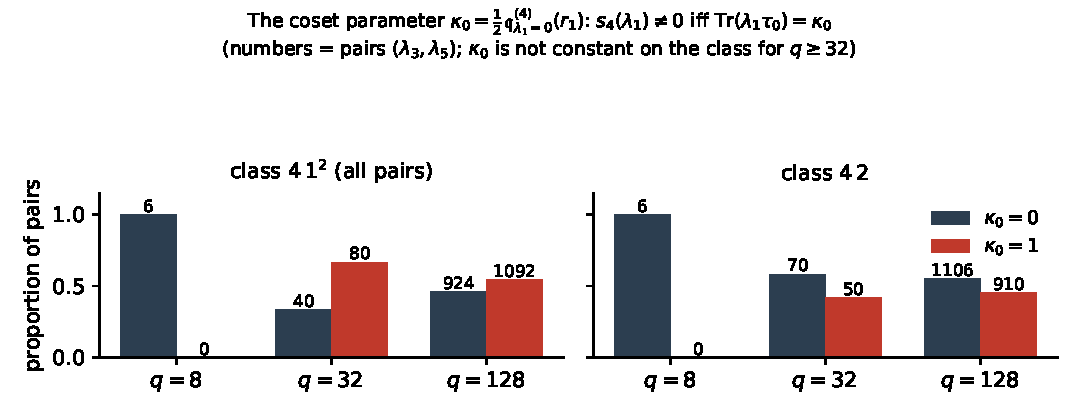
\includegraphics[width=\textwidth]{figures/fig4_kappa.pdf}
\caption{Proportion of pairs with $\kappa_0=0$ and $\kappa_0=1$ in the two classes of order $4$ (Table~\ref{tab:kappa}).}\label{fig:kappa}
\end{figure}

\begin{lemma}[the locus of the classes of order $4$]\label{lem:resolvent}
Let $k$ be odd. In the coordinates $y\in\F_q\setminus\{0,1\}$, $s\in\F_q^\times$ of the proof of Proposition~\ref{prop:kappa} ($\tau_0=y^2+y$, $\rho_0=s\tau_0^2$, $z=y^4$, $b=\rho_0z/\tau_0$, $t=(y/(y+1))^4$), every pair $(a,b)$ whose sextic has a quadratic factor arises exactly once, and the substitution $u=\tau_0(x^{-1}+1)$ turns the quartic cofactor into the depressed quartic
\[
\Phi(x)=x^4+a'x^2+b'x+c',\qquad a'=\frac1{1+t},\quad b'=c'=\frac1{s(1+t)} .
\]
The pair is of class $4\,1^2$ or $4\,2$ iff $\Phi$ is irreducible over $\F_q$, iff the resolvent cubic $Y^3+a'Y+b'$ has exactly one root $r\in\F_q$ and
\[
\Tr_{q/2}\Bigl(\frac{c'}{(a'+r^2)^2}\Bigr)=1,\qquad \Tr_{q/2}\Bigl(\frac{a'}{r^2}\Bigr)=0 ;
\]
the class is $4\,1^2$ iff $\Tr_{q/2}(s)=0$.
\end{lemma}
\begin{proof}
The parametrisation is Lemma~\ref{lem:cofactor} (the two solutions $b$ of $\tau_0b^2+\rho_0b+\rho_0^2\tau_0^3=0$ correspond to $y$ and $y+1$). With $u=\tau_0w$ the cofactor becomes $w^4+w^3+(1+s)w^2+w+st$, with $w=x+1$ this is $x^4+x^3+sx^2+s(1+t)$, and reversing the coefficients gives $\Phi$. For the criterion (Berlekamp \cite{Berlekamp}, Leonard--Williams \cite{LeonardWilliams}): if $\alpha_1,\dots,\alpha_4$ are the roots of $\Phi$ ($\sum\alpha_i=0$), the three sums $\gamma=\alpha_i+\alpha_j$ ($=\alpha_l+\alpha_n$ for the complementary pair) are the roots of $Y^3+a'Y+b'$. A $4$-cycle fixes exactly one $\gamma$, say $r=\alpha_1+\alpha_3$; then $\Phi=(x^2+rx+\mu)(x^2+rx+\mu')$ with $\mu=\alpha_1\alpha_3$, $\mu'=\alpha_2\alpha_4$ the roots of $X^2+(a'+r^2)X+c'$, and $\Phi$ is irreducible iff $\mu\notin\F_q$ and $x^2+rx+\mu$ has no root in $\F_{q^2}$, i.e.\ iff $\Tr_{q/2}(c'/(a'+r^2)^2)=1$ and $\Tr_{q^2/2}(\mu/r^2)=\Tr_{q/2}((a'+r^2)/r^2)=1$, the latter being $\Tr_{q/2}(a'/r^2)=1+\Tr_{q/2}(1)=0$ for odd $k$. Conversely these conditions exclude the types $(2,2)$, $(1,1,2)$, $(1,3)$, $(1,1,1,1)$ (for which the cubic has three roots, or one root with the opposite trace values). The last assertion is the splitting criterion for $u^2+\tau_0u+\rho_0$. All statements are also verified for every $(y,s)$ at $q=8,32,128$ (\texttt{part4\_kappa\_scan.py}).
\end{proof}

\begin{remark}
The lemma describes the locus of the classes of order $4$ inside the $(y,s)$-plane by one cubic and two Artin--Schreier conditions, so the counts $n_{4\,1^2}+n_{4\,1^2}^{\rm pure}=(q-2)(q-4)/8+(q-2)/2$ and $n_{4\,2}=q(q-2)/8$ of Target Theorem~\ref{tgt:counts} are, in this parametrisation, point counts of an explicit curve of Artin--Schreier type over the cubic resolvent; this is a possible route to those two entries of the table that avoids the moments. The expectation of an earlier draft that the resolvent conditions would force $\kappa_0=0$ was wrong: $\kappa_0$ and the irreducibility conditions are independent trace conditions.
\end{remark}

\subsection{The classes with \texorpdfstring{$N_0\mid2$}{N0 | 2}}
The sixteen-term version of the hexad formula has a combinatorial structure that decides the sign completely. We first isolate it.

\begin{lemma}[the sixteen-point configuration]\label{lem:sixteen}
Let $m\in\{2,3\}$, suppose $T'^{-1}(1)=r_1+\Kk_\lambda\subset\F_{q^m}$ (all sixteen points rational over $\F_{q^m}$), and suppose all sixteen values $\qq^{(m)}_\lambda(w)$ have the same parity $p\in\{0,1\}$. Put $\phi(w)=(\qq^{(m)}_\lambda(w)-p)/2\in\F_2$ and $\phi_i=\phi(r_i)$. Then
\begin{enumerate}[label=\textup{(\roman*)},leftmargin=2em]
\item $\phi(r_i+r_j+r_l)=\phi_i+\phi_j+\phi_l$ for every total, and $\sum_{i=1}^6\phi_i=0$;
\item with $n_1=\#\{i:\phi_i=1\}$ (an even number),
\[
\sum_{i=1}^6(-1)^{\phi_i}-\sum_{w\ \mathrm{total}}(-1)^{\phi(w)}=\begin{cases}+4,& n_1\in\{2,6\},\\ -4,& n_1\in\{0,4\};\end{cases}
\]
\item consequently $s_{2m}(\lambda)=i^{p}\,q^m\cdot(\pm4)$ with the sign of \textup{(ii)}; in particular $s_{2m}\ne0$.
\end{enumerate}
\end{lemma}
\begin{proof}
(i) For $\kappa\in\Kk_\lambda$ and $w\in T'^{-1}(1)$, \eqref{eq:polar} gives $\qq(w+\kappa)=\qq(w)+\qq(\kappa)+2\Tr_{q^m/2}(\kappa)$, where $\qq(\kappa)$ is even ($\kappa$ is a difference of two coset points of equal parity) and $\qq$ is additive on $\Kk_\lambda$ (Lemma~\ref{lem:gaussbasics}(i), $\Kk_\lambda\subset\F_{q^m}$ being the radical). So $\psi(\kappa):=\frac12\qq(\kappa)+\Tr_{q^m/2}(\kappa)$ is an $\F_2$-linear functional on $\Kk_\lambda$ and $\phi(w+\kappa)=\phi(w)+\psi(\kappa)$. For a duad, writing $\qq(r_i)=p+2\phi_i$ and using $T'(r_i)=1$, $\Tr_{q^m/2}(r_j)\equiv\qq(r_j)\equiv p$:
\[
\qq(r_i+r_j)=\qq(r_i)+\qq(r_j)+2\Tr_{q^m/2}(r_j)\equiv2p+2\phi_i+2\phi_j+2p\equiv2(\phi_i+\phi_j)\pmod4,
\]
so $\psi(r_i+r_j)=\phi_i+\phi_j+\Tr(r_i)+\Tr(r_j)=\phi_i+\phi_j+2p=\phi_i+\phi_j$. Hence $\phi(r_i+r_j+r_l)=\phi_i+\psi(r_j+r_l)=\phi_i+\phi_j+\phi_l$. Computing the same total through the complementary triple gives $\sum_{i=1}^6\phi_i=0$; equivalently, $\qq(\sum r_i)=\qq(0)=0$ expanded by \eqref{eq:polar}.
(ii) $\sum_i(-1)^{\phi_i}=6-2n_1$. The ten totals correspond to the ten partitions of $\{1,\dots,6\}$ into two triples, and the sign of a total is $(-1)^{t}$ with $t$ the number of indices with $\phi=1$ in either triple ($t$ and $n_1-t$ have the same parity as $n_1$ is even). For $n_1=0$: all totals $+$, total $6-10=-4$. For $n_1=2$: the two indices lie in the same triple for $4$ partitions ($+$) and are separated for $6$ ($-$): $2-(4-6)=+4$. For $n_1=4,6$ replace $\phi$ by $\phi+1$, which negates both sums. (iii) is Theorem~\ref{thm:hexadformula}.
\end{proof}

\begin{theorem}[the classes with $N_0\mid2$]\label{thm:N0div2}
Let $k$ be odd and $B_\lambda$ of class $1^6$, $2\,1^4$, $2^21^2$ or $2^3$. For every $\lambda_1$ all sixteen values $\qq^{(2)}_\lambda(w)$, $w\in T'^{-1}(1)$, are even; put $\phi_i=\frac12\qq^{(2)}_\lambda(r_i)$. Then $s_4(\lambda_1)=\pm4q^2$ with the sign of Lemma~\ref{lem:sixteen}\textup{(ii)}, where:
\begin{enumerate}[label=\textup{(\roman*)},leftmargin=2em]
\item every rational root has $\phi_i=\Tr_{q/2}(r_i)=f_1(C)+1$, and conjugate roots have equal $\phi_i$;
\item class $1^6$: $n_1=6$ and $s_4(\lambda_1)=+4q^2$ for all $\lambda_1$;
\item class $2^3$: the number of conjugate pairs with $\phi=1$ is odd, $n_1\in\{2,6\}$, and $s_4(\lambda_1)=+4q^2$ for all $\lambda_1$;
\item class $2\,1^4$ (rational roots $r_1,\dots,r_4$, pair $r_5,r_6$, $\tau_0=r_5+r_6$): $n_1=2\phi_5$ and $s_4(\lambda_1)=+4q^2$ iff $\frac12\qq^{(2)}_\lambda(r_5)=1$, which holds for exactly $q/2$ values of $\lambda_1$ (those with $\Tr_{q/2}(\lambda_1\tau_0)=1+\frac12\qq^{(2)}_{\lambda,0}(r_5)$);
\item class $2^21^2$ (rational roots $r_1,r_2$, pairs $\{r_3,r_4\}$, $\{r_5,r_6\}$): $n_1=2+2\phi_3+2\phi_5$ and $s_4(\lambda_1)=+4q^2$ iff $\phi_3=\phi_5$, which holds for exactly $q/2$ values of $\lambda_1$ (those with $\Tr_{q/2}(\lambda_1(r_1+r_2))=\frac12\qq^{(2)}_{\lambda,0}(r_3)+\frac12\qq^{(2)}_{\lambda,0}(r_5)$).
\end{enumerate}
In particular $W'=+4q^7$ in the classes $1^6$, $2^3$ and $W'=0$ in the classes $2\,1^4$, $2^21^2$: Target Theorem~\ref{tgt:signs} holds for the six classes with $N_0\mid4$.
\end{theorem}
\begin{proof}
\emph{Parity.} Theorem~\ref{thm:traceparity} with $m=2$, $2k+f_2=2k+4$ even, once its hypothesis is checked: $\Kk_\lambda\cap\ker\tau_2=\Kk_\lambda\cap\F_q=\Kk_\lambda^\sigma$ is spanned by the duads fixed by $\sigma$, i.e.\ $r+\sigma r$ for a conjugate pair and $r_i+r_j$ for two rational roots, and $\qq^{(2)}_{\lambda,0}$ vanishes on them: $\qq^{(2)}(r+\sigma r)=2\qq^{(2)}(r)+2\Tr_{q^2/2}(r)\equiv2(\qq^{(2)}(r)+\Tr_{q^2/2}(r))=0$ by Lemma~\ref{lem:gaussbasics}(ii), and $\qq^{(2)}(r_i+r_j)=2\Tr_{q/2}(r_i+r_j)=0$ for rational $r_i,r_j$ by the pair lemma (for $x\in\F_q$, $\qq^{(2)}_\lambda(x)=2\Tr_{q/2}(x)$ as in Step~1 of Theorem~\ref{thm:hexadformula}). So Lemma~\ref{lem:sixteen} applies with $p=0$.

(i) For rational $r$, $\qq^{(2)}_\lambda(r)=2\Tr_{q/2}(r)$ for every $\lambda_1$, and $\Tr_{q/2}(r)=f_1+1$ by Corollary~\ref{cor:rationalroots}; $\qq^{(2)}_\lambda$ is $\sigma$-invariant. (ii) $f_1(1^6)=4$. (iii) $f_1(2^3)=2$; the four rational points of the coset are totals (the partitions $\{1,3,5\}|\{2,4,6\}$ etc.\ with one index from each pair, which $\sigma=(12)(34)(56)$ maps to their complements), and such a total $w=r_a+r_b+r_c$ has $\phi(w)=\Tr_{q/2}(w)=f_1+1=1$ by Corollary~\ref{cor:rationalroots} (totals included) and $\phi(w)=\phi_a+\phi_b+\phi_c$ by Lemma~\ref{lem:sixteen}(i), one $\phi$ from each pair; hence an odd number of pairs has $\phi=1$. (iv), (v): $f_1=3$, resp.\ $2$, give $\phi=0$, resp.\ $1$, at the rational roots, and the pairs contribute $0$ or $2$ to $n_1$; the $\lambda_1$-dependence is $\frac12\qq^{(2)}_{\lambda}(r)=\frac12\qq^{(2)}_{\lambda,0}(r)+\Tr_{q/2}(\lambda_1\tau_2(r))$ with $\tau_2(r_5)=\tau_0\ne0$ in (iv) and $\tau_2(r_3)+\tau_2(r_5)=r_3+r_4+r_5+r_6=r_1+r_2\ne0$ in (v), so each sign occurs for $q/2$ values of $\lambda_1$. The values of $W'=q^4\sum_{\lambda_1}s_4$ follow, and the statement about Target Theorem~\ref{tgt:signs} combines this with Theorem~\ref{thm:order4}.
\end{proof}

\begin{remark}
(1) Table~\ref{tab:hexadterms} is the theorem at $q=8$: e.g.\ in the class $2^21^2$ the rational roots always have $\phi=1$ (``$2{:}2$'' among the roots), and the three patterns are $n_1=2,4,6$ with signs $+,-,+$; in the class $2^3$ the patterns are $n_1=2$ and $n_1=6$. The rule is verified for every pair and every $\lambda_1$ at $q=8$ and for three pairs per class at $q=32$ (\texttt{part4\_sign\_rules.py}). (2) The proof explains the ``half-half'' behaviour of the classes $2\,1^4$ and $2^21^2$ and the constancy in the classes $1^6$, $2^3$ in one stroke: a conjugate pair contributes an even number to $n_1$ and its $\phi$ depends on $\lambda_1$ through $\Tr(\lambda_1\tau)$, $\tau$ the sum of the pair; in the classes $1^6$ and $2^3$ these $\tau$'s sum to zero over the pairs, so $n_1\bmod4$ is independent of $\lambda_1$, while in the other two classes exactly one $\tau$ (resp.\ one sum of two $\tau$'s) is free.
\end{remark}

\subsection{The classes with \texorpdfstring{$N_0\in\{3,6\}$}{N0 in \{3,6\}}}\label{subsec:N0div6}
For $N_0\in\{3,6\}$ the relevant small field is $\F_{q^3}$ and the relevant hypothesis of Theorem~\ref{thm:traceparity} is
\begin{equation}\label{eq:H}
\textup{(H)}\qquad s_3(\lambda_1')\ne0\ \text{for some }\lambda_1'\in\F_q,\quad\text{i.e.\ }\tfrac12\qq^{(3)}_{\lambda,0}\ \text{vanishes on }\Kk_\lambda\cap\F_{q^3}\cap\ker\tau_3
\end{equation}
(Lemma~\ref{lem:gaussbasics}(iv)).

\begin{lemma}\label{lem:Hcheck}
\textup{(H)} holds unconditionally in the classes $3\,1^3$ and $3^2$. In the class $6$ it is equivalent to the single identity $\qq^{(3)}_{\lambda,0}(r_1+r_4)=0$, $r_4=\sigma^3r_1$, which does not depend on $\lambda_1$ and is equivalent to $\Tr_{q^3/2}(N\gamma_w)=1$ for $w=r_1+r_4$, $N=r_1r_4$, $\gamma_w=1+\lambda_5w^3+\lambda_3w+(\lambda_5w)^{1/2}$; it holds for all pairs of the class at $q=8$ and $q=32$.
\end{lemma}
\begin{proof}
For a duad inside a $\sigma$-orbit contained in $\F_{q^3}$, $\qq^{(3)}(r+\sigma r)=2\qq^{(3)}(r)+2\Tr_{q^3/2}(r)\equiv0$ by Lemma~\ref{lem:gaussbasics}(ii). Class $3\,1^3$ ($\sigma=(123)$): $\tau_3$ vanishes on the duads $r_1+r_2$, $r_2+r_3$, $r_1+r_3$ and is $\ne0$ on the twelve others ($\tau_3(r_4+r_5)=r_4+r_5$, $\tau_3(r_1+r_4)=r_5+r_6$), so $\Kk_\lambda\cap\ker\tau_3=\{0,r_1+r_2,r_2+r_3,r_1+r_3\}$, on which $\qq^{(3)}_0$ vanishes by the first sentence. Class $3^2$ ($\sigma=(123)(456)$, $\alpha:=r_1+r_2+r_3=r_4+r_5+r_6\in\F_q$): $\tau_3\equiv0$ on $\Kk_\lambda$, and it remains to treat a duad $r_1+r_4$ across the two cycles. With $\beta=e_2(r_1,r_2,r_3)$, $\beta''=e_2(r_4,r_5,r_6)$ and $\beta+\beta''+\alpha^2=e_2(r_1,\dots,r_6)=0$,
\begin{align*}
\Tw_{3k}(r_1)+\Tw_{3k}(r_4)&=\bigl(\Tw_k(\alpha)+2\Tr(\beta)\bigr)+\bigl(\Tw_k(\alpha)+2\Tr(\beta+\alpha^2)\bigr)\\
&=2\Tw_k(\alpha)+2\Tr(\alpha)=4\Tr(\alpha)+4e_2^{\rm abs}(\alpha)\equiv0\pmod 4,
\end{align*}
and $2\Tr_{q^3/2}\bigl(f(r_1)+f(r_4)\bigr)=2\Tr_{q/2}\bigl(\lambda_5p_5+\lambda_3p_3+2\lambda_1\alpha\bigr)$ with $p_3,p_5$ the power sums of all six roots, which are $p_3=0$ and $p_5=5e_5=b$ (Newton with $e_1=e_2=e_3=0$); so this is $2\Tr(\lambda_5b)=2\Tr(1)=2$. By \eqref{eq:polar}, $\qq^{(3)}_0(r_1+r_4)=\qq^{(3)}_0(r_1)+\qq^{(3)}_0(r_4)+2\Tr_{q^3/2}(r_4)=2+2\Tr_{q/2}(\alpha)$. Now $\alpha$ is a synthematic total ($\{123\}|\{456\}$), rational, so $\Tr_{q/2}(\alpha)=f_1(3^2)+1=1$ by Corollary~\ref{cor:rationalroots}, and $\qq^{(3)}_0(r_1+r_4)=0$. Class $6$: $\Kk_\lambda\cap\F_{q^3}=\Kk_\lambda^{\sigma^3}=\{0,r_1+r_4,r_2+r_5,r_3+r_6\}$, on which $\tau_3$ vanishes ($\tau_3(r_1+r_4)=\sum r_i=0$) and which is permuted by $\sigma$, so (H) is the one identity stated. For the reformulation apply Step~3 of the proof of Theorem~\ref{thm:hexadformula} to $c=r_1$, $c+c^{q^3}=w$, which gives $\qq^{(6)}_\lambda(r_1)=\qq^{(3)}_\lambda(w)+2\Tr_{q^3/2}(N\gamma_w)$ (that step used nothing about $T'(w)$), together with $\qq^{(6)}_\lambda(r_1)=\Tw_{6k}(r_1)+2\Tr_{q^6/2}(f(r_1))=\Tr_{W_2(\F_q)/\Z/4}(e_1,e_2)+2\Tr_{q/2}(\lambda_5p_5+\lambda_3p_3+\lambda_1p_1)=0+2\Tr(\lambda_5b)=2$. The numerical statement is Part~III, Table~7 ($q=8$) and the $L$-polynomial data of Part~III at $q=32$ (\texttt{witt\_lpoly\_k5.txt}: $s_3\ne0$ for all $128$ triples of the class), and \texttt{part4\_sign\_rules.py}.
\end{proof}

\begin{theorem}[the classes with $N_0\in\{3,6\}$]\label{thm:N0div6}
Let $k$ be odd.
\begin{enumerate}[label=\textup{(\roman*)},leftmargin=2em]
\item In the classes $3\,1^3$ and $3^2$, for every $\lambda_1$: all sixteen values $\qq^{(3)}_\lambda(w)$, $w\in T'^{-1}(1)$, are odd, $s_6(\lambda_1)=\pm4i\,q^3$ with the sign of Lemma~\ref{lem:sixteen}\textup{(ii)} applied to $\phi(w)=(\qq^{(3)}_\lambda(w)-1)/2$, and $\Spp(\lambda_1)=+4q^6$. Hence $W'=+4q^7$.
\item In the class $6$, assume \textup{(H)}. Then for every $\lambda_1$ the four values $\qq^{(3)}_\lambda(w)$ at the points of $T'^{-1}(1)\cap\F_{q^3}$ (four synthematic totals) are odd and equal, $s_6(\lambda_1)=\mp4i\,q^3$ accordingly, and $\Spp(\lambda_1)=+4q^6$, $W'=+4q^7$.
\item In the class $3\,2\,1$, assume \textup{(H)}. Then every $w\in T'^{-1}(1)\cap\F_{q^3}$ (four roots and four totals) has $\Tr_{q^3/2}(w)=0$, all terms of \eqref{eq:hexadformula} are $\pm1$, and $s_6(\lambda_1)\in\{0,\pm4q^3\}$.
\end{enumerate}
\end{theorem}
\begin{proof}
(i) By Lemma~\ref{lem:Hcheck}, Theorem~\ref{thm:traceparity} applies with $m=3$ and $3k+f_3=3k+4$ odd: every coset point in $\F_{q^3}$ (all sixteen) has odd Witt value. Lemma~\ref{lem:sixteen} with $p=1$ gives $s_6=i\,q^3(\pm4)$, in particular $s_6\ne0$ and $\nu_6=-s_6/4q^3=\mp i$; by Part~III, Theorem~6.14(iii), $\Spp=-4q^6\nu_6^2=+4q^6$. (ii) Trace parity with $3k+f_3=3k+2$ odd gives odd values at the four points $w_0+\Kk_\lambda^{\sigma^3}$; by \eqref{eq:polar} and (H), $\qq^{(3)}(w_0+\kappa)=\qq^{(3)}(w_0)+\qq^{(3)}(\kappa)+2\Tr_{q^3/2}(\kappa)=\qq^{(3)}(w_0)+0+2\Tr_{q/2}(\tau_3\kappa)=\qq^{(3)}(w_0)$ for $\kappa\in\Kk_\lambda^{\sigma^3}$ (the $\lambda_1$-part of $\qq^{(3)}(\kappa)$ is $2\Tr_{q/2}(\lambda_1\tau_3\kappa)=0$). So the four terms of \eqref{eq:hexadformula} are equal, all with $\eps=-1$: $s_6=-4q^3\,i^{\qq^{(3)}(w_0)}=\mp4iq^3$, and $\Spp=+4q^6$ as before. (iii) Trace parity with $3k+f_3=3k+3$ even.
\end{proof}

\begin{remark}
(1) Theorem~\ref{thm:N0div6}(i) settles Target Theorem~\ref{tgt:signs} for the classes $3\,1^3$ and $3^2$, and (ii) for the class $6$ modulo the single Witt identity (H), which is verified for all pairs at $q=8$ and $q=32$. Together with Theorems~\ref{thm:order4} and \ref{thm:N0div2}, nine of the eleven classes are done unconditionally and one conditionally; Table~\ref{tab:hexadterms} is the theorem at $q=8$ (class $3^2$: $n_1\in\{0,6\}$ only, because $\psi\equiv0$ there; class $3\,1^3$: all four values of $n_1$ occur). (2) The class $3\,2\,1$ remains open: (iii) is consistent with the target ($\Spp=\pm4q^6$ in equal numbers) but does not prove it, because when $s_6(\lambda_1)=0$, which happens (Table~\ref{tab:hexadterms}), $\Spp(\lambda_1)$ is not determined by $s_6$; one needs either $s_{12}$ directly or the $L$-polynomial from $s_1,\dots,s_4$ as in Part~III. (3) Figure~\ref{fig:phases} shows the normalised Frobenius eigenvalues of the Witt sheaf at $q=8$ in all classes; the order-$4$ classes are rotated against each other by $2\pi/8$, which is the sign $(-1)^{\Tr(\rho_0/\tau_0^2)}$ of Theorem~\ref{thm:order4} seen on the eigenvalues ($\omega_j^4=-q^2\,\sgn s_4$).
\end{remark}

\begin{figure}[htbp]
\centering
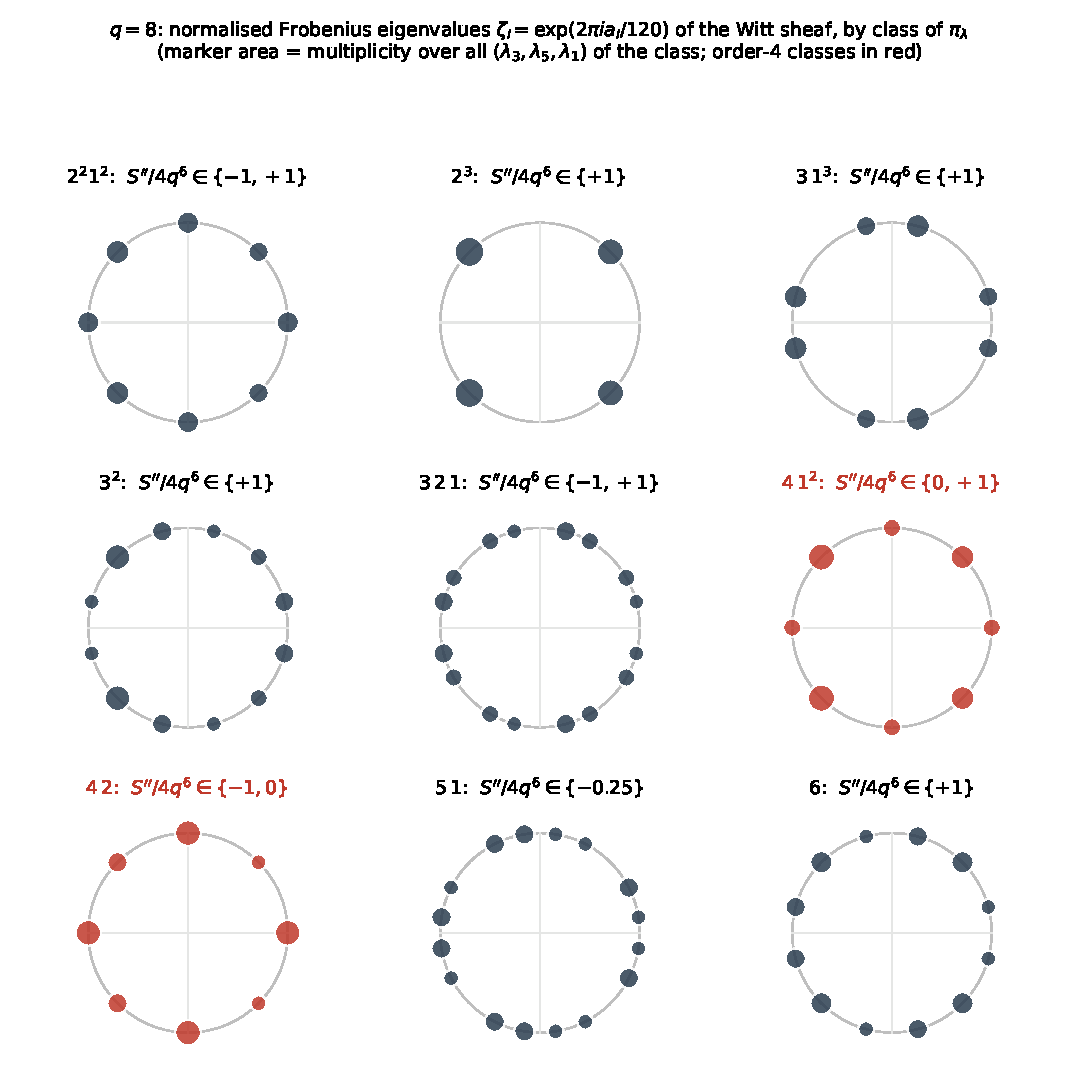
\includegraphics[width=0.96\textwidth]{figures/fig4_phases.pdf}
\caption{Normalised Frobenius eigenvalues $\zeta_j=\omega_j/\sqrt q$ of the rank-$4$ Witt sheaf at $q=8$, by class of $\pi_\lambda$ (from the $L$-polynomial data of Part~III, \texttt{witt\_lpoly\_k3\_b120.txt}); marker area is proportional to multiplicity over all $(\lambda_3,\lambda_5,\lambda_1)$ of the class. The two classes of order $4$ (red) have $\{\zeta_j\}=\zeta_8^{\pm1}\cdot\mu_4$ and $\mu_4$ respectively (plus the eigenvalues of the $\lambda_1$ with $s_4=0$), the mirror image under rotation by $2\pi/8$ predicted by Theorem~\ref{thm:order4}.}\label{fig:phases}
\end{figure}

\section{The constant \texorpdfstring{$X$}{X}}\label{sec:X}
\begin{theorem}\label{thm:Xstatus}
Let $k$ be odd. Suppose that Target Theorem~\ref{tgt:counts} holds, that \textup{(H)} of \eqref{eq:H} holds in the class $6$, and that
\begin{enumerate}[label=\textup{(\alph*)},leftmargin=2em]
\item $\Spp(\lambda_1)=+4q^6$ for exactly $q/2$ values of $\lambda_1$ in the class $3\,2\,1$ (equivalently $W'=0$ there).
\end{enumerate}
Then $X=q^6+q^5$ and the variance formula of Corollary~\ref{cor:X} holds. Of the eleven sign hypotheses of Part~III, Corollary~1.5, only (a) and \textup{(H)} remain (Theorems~\ref{thm:order4}, \ref{thm:N0div2}, \ref{thm:N0div6}).
\end{theorem}
\begin{proof}
Under (a), (H) and Theorems~\ref{thm:order4}, \ref{thm:N0div2}, \ref{thm:N0div6} the values of $W'$ on the classes are those of Part~III, Theorem~6.9 ($+4q^7$, $0$, $0$, $+4q^7$, $+4q^7$, $+4q^7$, $0$, $+2q^7$, $-2q^7$, $-q^7$, $+4q^7$ in the order of Table~\ref{tab:classes}), and the bookkeeping of Part~III, Corollary~1.5, with the counts of Target Theorem~\ref{tgt:counts} gives $q^3X=W'(0,0)+\sum_{\lambda_3\ne0}W'(\lambda_3,0)+\sum_{\lambda_5\ne0,\lambda_3=0}W'+\sum_{\text{mixed}}W'=q^7+q^8+(3q^8-2q^7)+(q^9-3q^8+q^7)=q^9+q^8$.
\end{proof}

\begin{remark}[even $k$]
For even $k$ Part~III (\S6.11, Table~9) gives $X=-q^6+q^5$ with class counts depending on $k\bmod4$. The hexad formula and Lemma~\ref{lem:gaussbasics} hold verbatim; the trace parity theorem changes by the term $mk$ (even), so rational roots have trace $f_1(C)\bmod2$; in Theorem~\ref{thm:order4} the roles of the two classes are then \emph{exchanged} ($\Tr(r_5)=1$ in $4\,1^2$, $\Tr(w_3)=1$ in $4\,2$), giving $s_4\in\{0,-4q^2\}$ in $4\,1^2$ and $\{0,+4q^2\}$ in $4\,2$, i.e.\ $W'=-2q^7$ and $+2q^7$, in agreement with the sign $(-1)^{k+1}$ in front of $q^6$ observed in Part~II and with the values $W'=\mp2q^7$ found at $q=4$ in Part~III, \S6.11. At $q=4$ the four pairs of the classes $4\,1^2$, $4\,2$ indeed have $s_4\in\{0,-4q^2\}$, resp.\ $\{0,+4q^2\}$, on the hyperplane $\Tr(\lambda_1\tau_0)=\kappa_0$, with $W'=-2q^7$, resp.\ $+2q^7$ (\texttt{part4\_order4\_all.py 2}). The even-$k$ form of Corollary~\ref{cor:rationalroots}, $\Tr_{q/2}(r)\equiv f_1(C)\pmod2$, is verified for every rational root at $q=4,16,64$ (\texttt{part4\_trace\_parity.py}: e.g.\ all $1024$ rational roots of the class $4\,1^2$ at $q=64$ have trace $1$, all $819$ of the class $5\,1$ have trace $0$).
\end{remark}

\section{Supersingular abelian surfaces, canonical lifts and the hexad}\label{sec:lifts}
This section is expository and contains no theorems; it records the interpretation of the structures above that the authors regard as most likely, and the questions it raises (Part~III, Open Problems~4 and~6).

\subsection{The hexad as $2$-torsion of a lift}
The six roots of $B_\lambda$ do not depend on $\lambda_1$; they are attached to the supersingular curve $C_\lambda:y^2+y=\lambda_5x^5+\lambda_3x^3$ of genus $2$, whose Jacobian $J_\lambda$ is a supersingular abelian surface (van der Geer--van der Vlugt \cite{vdGvdV}; for the classification of supersingular abelian surfaces see Oort \cite{Oort}). The symplectic $\F_2$-space $(\Kk_\lambda,\omega)$ of Part~III has automorphism group $\Sp_4(\F_2)\cong S_6$ \cite{Atlas}, the six roots behave as the six Weierstrass points of a genus-two curve (the totals as the ten even theta characteristics, the duads as the fifteen nonzero $2$-torsion points), and the Frobenius acts through $S_6$ as $\pi_\lambda$. In characteristic $2$ the Jacobian of a supersingular curve has no \'etale $2$-torsion, so $(\Kk_\lambda,\omega)$ cannot be $J_\lambda[2](\bar\F_q)$. It can be the $2$-torsion of a \emph{lift}: by the theory of Serre and Tate \cite{LST,KatzST} every ordinary abelian variety has a canonical lift to $W(\F_q)$; for supersingular ones there are the quasi-canonical lifts of Gross \cite{Gross} and, more generally, lifts to finite extensions of $W(\F_q)$ whose generic fibre is an abelian surface $\tilde J$ with $\tilde J[2]\cong(\Z/2)^4$ carrying the Weil pairing and a Galois action through $\Sp_4(\F_2)$. The Witt vectors of length two, which are the natural home of the forms $\qq^{(m)}_\lambda$ (they are $\Z/4$-valued because $W_2(\F_2)=\Z/4$), are the mod-$4$ reduction of this lifting ring, and the Dieudonn\'e crystal of $J_\lambda$ reduced modulo $2$ is where $\Kk_\lambda$ should live. The hexad formula (Theorem~\ref{thm:hexadformula}) fits this picture: a Gauss sum over $\F_{q^{2m}}$ is computed by a sum over the $\F_{q^m}$-rational $2$-torsion-like points (roots and totals) of the lift, with the sign $\eps$ distinguishing the ``odd'' from the ``even'' points, exactly as the theta constants of a genus-two curve distinguish the six odd from the ten even characteristics; the trace parity theorem is then a statement about the field of definition of these points.

\subsection{The role of $\mu_5$ and the dependence on $k\bmod 4$}
For even $k$ the class counts of Part~III, Table~9, depend on $k\bmod4$ through the classes $1^6$, $2^21^2$, $5\,1$ and the pure column, while for odd $k$ they do not. The mechanism is the splitting of the fifth roots of unity: $\mu_5\subset\F_q$ iff $4\mid k$, $\F_q(\mu_5)=\F_{q^2}$ for $k\equiv2\bmod4$, and $\F_q(\mu_5)=\F_{q^4}$ for odd $k$ regardless of $k\bmod 4$. The class $5\,1$ corresponds to a quintic factor of $B_\lambda$ whose splitting field is $\F_{q^5}$ and whose Galois group, a $5$-cycle, is the image of a Kummer-type extension generated by a fifth root once $\mu_5$ is adjoined; the $5$-cycles form one class in $S_6$ but two in $A_6$, and which of the two occurs is governed by $\mathrm{Gal}(\F_q(\mu_5)/\F_q)$. Through the moment identities (Proposition~\ref{prop:elimination}) the branching of $n_{5\,1}$ along $k\bmod4$ propagates to $1^6$ and $2^21^2$. In the picture of the previous paragraph, $\mu_5$ enters through the automorphism $x\mapsto\zeta_5x$ of the pure curves $y^2+y=\lambda_5x^5$ (complex multiplication by $\Z[\zeta_5]$ on the lift), and the decomposition group of $5$ in $\Q(\zeta_5)/\Q$ at the prime $2$ (which has order $4$) is what makes $m=5$ special in the moment system: the row $m=5$ of Proposition~\ref{prop:elimination} is the only one whose Gauss-sum total $\Sigma_5=q^3(q^2+1)$ involves $q^2+1=(q+i)(q-i)$, the norm form of the splitting of $2$ in $\Q(i)\subset\Q(\zeta_{20})$, and the only one in which $f^{(5)}$ separates the class $5\,1$ from all others. A proof of the even-$k$ counts would identify the relevant Kummer extension explicitly; the odd-$k$ counts, where $\F_q(\mu_5)$ is always $\F_{q^4}$, are the case without branching.

\section*{Computations}
All scripts are in the directory \texttt{code/} of the repository and depend only on NumPy, SymPy and Numba (for the field tables); their outputs are in \texttt{data/}, the figures are produced by \texttt{paper/make\_figures4.py}.
\begin{itemize}[leftmargin=2em]
\item \texttt{moment3\_check.py}: Proposition~\ref{prop:N3} and Conjecture~\ref{conj:N3value} for $q=8,32,128$.
\item \texttt{moment3\_structure.py}: Proposition~\ref{prop:GHstructure}.
\item \texttt{part4\_moment\_system.py}: Proposition~\ref{prop:elimination} and the interpolation checks.
\item \texttt{part4\_hexad\_formula.py}: Theorem~\ref{thm:hexadformula} for every $\lambda$ at $q=8$ ($m=2,3$) and for three pairs per class with $N_0\mid4$ at $q=32$ ($m=2$); Table~\ref{tab:hexadterms}.
\item \texttt{part4\_trace\_parity.py}: Corollary~\ref{cor:rationalroots} for every $(a,b)$ at $q=8,32,128$ (and $q=4,16,64$ for even $k$).
\item \texttt{part4\_sign\_rules.py}: Lemma~\ref{lem:sixteen} and Theorems~\ref{thm:N0div2}, \ref{thm:N0div6} ($\phi$-values with the Frobenius orbit structure, $n_1$, predicted and actual $s_{2m}$, hypothesis (H)) for every pair and every $\lambda_1$ at $q=8$ and three pairs per class at $q=32$.
\item \texttt{part4\_order4\_all.py}: for every pair of the classes of order $4$ at $q=8$ and $q=32$, the direct Witt values, $\kappa_0$ by \eqref{eq:q4r1} and \eqref{eq:kappaclosed}, and $s_4(\lambda_1)$ for all $\lambda_1$ (sign, hyperplane, $W'$).
\item \texttt{part4\_kappa\_scan.py}: Table~\ref{tab:kappa} and Lemma~\ref{lem:resolvent}; \texttt{part4\_relative\_reduction.py}: the coset form of the hexad formula; \texttt{part4\_brown\_invariants.py}: the earlier sampling version.
\end{itemize}

\section*{Acknowledgements}
The computations were carried out with NumPy and SymPy. The exploration that led to the hexad formula and to the trace parity theorem was carried out in an interactive session with Claude (Anthropic), which also assisted with the drafting of the manuscript; all proofs were checked by hand and all numerical statements by the scripts above.

\begin{thebibliography}{99}
\bibitem{Arf} C.~Arf, \emph{Untersuchungen \"uber quadratische Formen in K\"orpern der Charakteristik 2. I}, J. Reine Angew. Math. \textbf{183} (1941), 148--167.
\bibitem{Berlekamp} E.~R. Berlekamp, \emph{Algebraic Coding Theory}, McGraw-Hill, New York, 1968.
\bibitem{Bluher} A.~W. Bluher, \emph{On $x^{q+1}+ax+b$}, Finite Fields Appl. \textbf{10} (2004), 285--305.
\bibitem{Brown} E.~H. Brown, Jr., \emph{Generalizations of the Kervaire invariant}, Ann. of Math. (2) \textbf{95} (1972), 368--383.
\bibitem{Brylinski} J.-L. Brylinski, \emph{Th\'eorie du corps de classes de Kato et rev\^etements ab\'eliens de surfaces}, Ann. Inst. Fourier (Grenoble) \textbf{33} (1983), no.~3, 23--38.
\bibitem{Carlitz} L.~Carlitz, \emph{Kloosterman sums and finite field extensions}, Acta Arith. \textbf{16} (1969), 179--193.
\bibitem{Chen} R.~Chen, \emph{Primes in Legendre intervals over $\F_q[t]$: an exact explicit-formula algorithm, verification for $d\le10$, and an anomaly in characteristic~2}, preprint (2026), DOI 10.5281/zenodo.23225896.
\bibitem{ChenII} R.~Chen, \emph{Prime polynomials in Legendre intervals over $\F_{2^k}[t]$, II: exact variances via quadratic towers and supersingular Artin--Schreier curves}, preprint, version 2 (2026), DOI 10.5281/zenodo.23252762.
\bibitem{ChenIII} R.~Chen, \emph{Prime polynomials in Legendre intervals over $\F_{2^k}[t]$, III: the hexad of a quartic linearised polynomial, the symplectic group $\Sp_4(\F_2)$, and the Witt sums behind the constant $X$}, preprint (2026), DOI 10.5281/zenodo.23290724.
\bibitem{Atlas} J.~H. Conway, R.~T. Curtis, S.~P. Norton, R.~A. Parker, R.~A. Wilson, \emph{Atlas of Finite Groups}, Oxford University Press, 1985.
\bibitem{Deligne} P.~Deligne, \emph{La conjecture de Weil. II}, Inst. Hautes \'Etudes Sci. Publ. Math. \textbf{52} (1980), 137--252.
\bibitem{vdGvdV} G.~van der Geer, M.~van der Vlugt, \emph{Reed--Muller codes and supersingular curves. I}, Compositio Math. \textbf{84} (1992), 333--367.
\bibitem{Gross} B.~H. Gross, \emph{On canonical and quasi-canonical liftings}, Invent. Math. \textbf{84} (1986), 321--326.
\bibitem{HellesethKholosha} T.~Helleseth, A.~Kholosha, \emph{On the equation $x^{2^l+1}+x+a=0$ over $\mathrm{GF}(2^k)$}, Finite Fields Appl. \textbf{14} (2008), 159--176.
\bibitem{KatzST} N.~M. Katz, \emph{Serre--Tate local moduli}, in: Algebraic Surfaces (Orsay, 1976--78), Lecture Notes in Math. \textbf{868}, Springer, 1981, 138--202.
\bibitem{KatzKR} N.~M. Katz, \emph{Witt vectors and a question of Keating and Rudnick}, Int. Math. Res. Not. IMRN \textbf{2013}, no.~16, 3613--3638.
\bibitem{KatzEKR} N.~M. Katz, \emph{Witt vectors and a question of Entin, Keating, and Rudnick}, Int. Math. Res. Not. IMRN \textbf{2015}, no.~14, 5959--5975.
\bibitem{KeatingRudnick} J.~P. Keating, Z.~Rudnick, \emph{The variance of the number of prime polynomials in short intervals and in residue classes}, Int. Math. Res. Not. IMRN \textbf{2014}, no.~1, 259--288.
\bibitem{LachaudWolfmann} G.~Lachaud, J.~Wolfmann, \emph{The weights of the orthogonals of the extended quadratic binary Goppa codes}, IEEE Trans. Inform. Theory \textbf{36} (1990), 686--692.
\bibitem{LeonardWilliams} P.~A. Leonard, K.~S. Williams, \emph{Quartics over $\mathrm{GF}(2^n)$}, Proc. Amer. Math. Soc. \textbf{36} (1972), 347--350.
\bibitem{LidlNiederreiter} R.~Lidl, H.~Niederreiter, \emph{Finite Fields}, 2nd ed., Encyclopedia of Mathematics and its Applications \textbf{20}, Cambridge University Press, 1997.
\bibitem{LST} J.~Lubin, J.-P. Serre, J.~Tate, \emph{Elliptic curves and formal groups}, Lecture notes, Woods Hole Summer Institute, 1964.
\bibitem{Oort} F.~Oort, \emph{Which abelian surfaces are products of elliptic curves?}, Math. Ann. \textbf{214} (1975), 35--47.
\end{thebibliography}

\end{document}

